\newcommand{\DoNotLoadEpstopdf}{}
\documentclass[11pt]{article}
\usepackage[T1]{fontenc}
\usepackage{lmodern}
\usepackage[margin=1in]{geometry}
\usepackage{amsmath,amssymb,amsthm,mathtools}
\usepackage{microtype}
\usepackage{xcolor}
\usepackage{graphicx}
\usepackage{tikz}
\usetikzlibrary{arrows.meta,positioning,calc,decorations.pathreplacing}
\usepackage{enumitem}
\usepackage{needspace}
\usepackage[hyphens]{url}
\usepackage[colorlinks=true,linkcolor=blue!45!black,citecolor=green!35!black,urlcolor=blue!45!black]{hyperref}
\input{glyphtounicode.tex}
\input{glyphtounicode-cmex.tex}
\pdfgentounicode=1
\hypersetup{pdftitle={Annular variation of the triangular Hilbert transform at the symmetric point},pdfauthor={OpenAI}}
\newcommand{\R}{\mathbb R}
\newcommand{\C}{\mathbb C}
\newcommand{\dd}{\,\mathrm d}
\DeclareMathOperator{\tr}{tr}
\DeclareMathOperator{\diag}{diag}
\DeclareMathOperator{\supp}{supp}
\DeclareMathOperator{\Dil}{Dil}
\newcommand{\HS}{\mathrm{HS}}
\newcommand{\op}{\mathrm{op}}
\newtheorem{theorem}{Theorem}[section]
\newtheorem{proposition}[theorem]{Proposition}
\newtheorem{lemma}[theorem]{Lemma}
\newtheorem{corollary}[theorem]{Corollary}
\theoremstyle{definition}
\newtheorem{definition}[theorem]{Definition}
\theoremstyle{remark}
\newtheorem{remark}[theorem]{Remark}
\numberwithin{equation}{section}
\setlength{\emergencystretch}{2em}
\title{Annular variation of the triangular Hilbert transform\\at the symmetric point}
\author{OpenAI}
\date{October 5, 2026}
\begin{document}
\maketitle
\begin{abstract}
We prove the annular $r$-variation estimate for the triangular Hilbert
transform from complex $L^3\times L^3$ to $L^{3/2}$ for every $r>2$.
The partitions may depend on the output point and range over all positive
scales. The estimate yields the two-endpoint maximal bound and joint
almost-everywhere and norm principal values, and resolves the symmetric
scalar triangular Hilbert transform problem.
\end{abstract}
\tableofcontents
\section{Introduction}\label{sec:introduction}

For complex functions $F,G\in L^3(\R^2)$ and
$0<\varepsilon<R<\infty$, define the annular triangular Hilbert transform by
\begin{equation}\label{eq:bilinear-truncation}
 B_{\varepsilon,R}(F,G)(x,y)
 =\int_{\varepsilon<|t|<R}F(x+t,y)G(x,y+t)\,\frac{\dd t}{t}.
\end{equation}
The two inputs are translated along different coordinate directions.
Every finite integral is absolutely convergent outside one common
null set; we use its usual representative there and set all quantities
to zero on the exceptional set. Lemma~\ref{lem:finite-truncations}
justifies this convention and continuity in the endpoints.

For $r>2$, its annular variation is
\begin{equation}\label{eq:variation-definition}
 V_r(F,G)(x,y)
 =\sup_{\substack{J\ge1\,,\ 0<t_0<\cdots<t_J\\t_j\in\mathbb Q}}
    \left(\sum_{j=1}^J
          |B_{t_{j-1},t_j}(F,G)(x,y)|^r\right)^{1/r}.
\end{equation}
The supremum is pointwise: the partition may depend on $(x,y)$, and
there is no restriction on the number of endpoints within a dyadic
scale interval. The use of rational endpoints makes measurability
immediate and, by endpoint continuity, does not change the supremum.

\begin{theorem}[Full annular variation]\label{thm:variation}
For every real $r>2$ there is a finite constant $C_r$ such that
\[
 \|V_r(F,G)\|_{L^{3/2}(\R^2)}
 \le C_r\|F\|_{L^3(\R^2)}\|G\|_{L^3(\R^2)}
\]
for all complex $F,G\in L^3(\R^2)$.
\end{theorem}

Taking a single increment gives the maximal estimate with the supremum
over both hard truncation endpoints. In Section~\ref{sec:consequences}
we prove that the joint principal value
\[
 B(F,G)=\lim_{\substack{\varepsilon\downarrow0\\R\uparrow\infty}}
                   B_{\varepsilon,R}(F,G)
\]
exists almost everywhere and in $L^{3/2}$. In fact, the supremum of
$|B_{\varepsilon,R}(F,G)-B(F,G)|$ over
$0<\varepsilon<1/m$, $R>m$, tends to zero in $L^{3/2}$.

Pairing the bilinear output with a third $L^3$ input gives a scalar
form. Its symmetric, or simplex, coordinates are
\begin{equation}\label{eq:intro-simplex}
 \Lambda_{\varepsilon,R}(G_0,G_1,G_2)
 =\iiint_{\varepsilon<|a+b+c|<R}
  G_0(a,b)G_1(b,c)G_2(c,a)
             \frac{\dd a\dd b\dd c}{a+b+c}.
\end{equation}
The three equal exponents $3$ form the symmetric point of the scalar
H\"older relation $1/p_0+1/p_1+1/p_2=1$.
We obtain a uniform bound by $C\prod_v\|G_v\|_3$ and the joint scalar
principal value for every complex $L^3$ triple.
Proposition~\ref{prop:flat-equivalence} gives the norm-preserving
coordinate maps and equality of the optimal constants for the flat
and simplex scalar formulations. In particular, this proves the
symmetric scalar estimate in Thiele's Problem~13 in
\cite[Section~9]{GrafakosEtAl2017}.

\subsection{History and related work}

The flat operator occurs in Demeter and Thiele's study of bilinear
averages for two commuting transformations
\cite[Section~6]{DemeterThiele2010}. The scalar form
\eqref{eq:intro-simplex} is a basic entangled singular integral: each
input sees one pair of the three variables, and the pairs form a cycle.
This dependence differs from the bipartite configurations in many
multilinear estimates. Kova\v{c}, Thiele and Zorin-Kranich established
estimates for a Walsh model with two general inputs and a third input
of specified structure \cite[Theorem~1.7]{KovacThieleZorinKranich2015}.
Their paper also records the cyclic trace formulation and the
equivalence of the flat and simplex forms.

Quantitative cancellation over a finite range of scales was developed
in several stages. Tao proved sublogarithmic bounds for one-dimensional
multilinear Hilbert transforms \cite{Tao2016Cancellation}, and
Zorin-Kranich obtained sublogarithmic cancellation for simplex Hilbert
transforms \cite{ZorinKranich2017}. Durcik, Kova\v{c}, \v{S}kreb and
Thiele proved square-function and norm-variation estimates that yield
square-root cancellation for the triangular form over finitely many
smooth scales \cite[Corollary~5]{DurcikKovacSkrebThiele2019}.
Durcik, Kova\v{c} and Thiele obtained power-type cancellation for hard
truncations \cite[Theorem~1]{DurcikKovacThiele2019}. Permuting and
interpolating their $(4,4,2)$ bounds gives a
$\sqrt{\log(R/\varepsilon)}$ bound at the symmetric tuple.
These estimates retain a dependence on the scale range. Moreover,
norm-variation estimates for a fixed list of scales do not place the
supremum over output-dependent partitions inside the output norm as
in \eqref{eq:variation-definition}.

Other results gain cancellation by averaging a direction parameter
\cite{DurcikRoos2021,LinSlavikova2026} or by introducing curvature
\cite{ChristDurcikRoos2021,HsuLin2026}. Those mechanisms are distinct
from the flat problem considered here. The broader role of variation
in strengthening maximal estimates and controlling convergence is
illustrated by L\'epingle's martingale inequality
\cite{Lepingle1976}, the variational inequalities of Jones, Seeger and
Wright \cite{JonesSeegerWright2008}, and the variation-norm Carleson
theorem \cite{OberlinSeegerTaoThieleWright2012}. These results provide
context rather than an input to our proof.

The energy method here is related to telescoping arguments for
entangled forms: Kova\v{c}'s twisted paraproduct and Bellman-function
framework \cite{Kovac2012Twisted,Kovac2011}, and Durcik's continuous
Gaussian telescoping \cite{Durcik2015,Durcik2017}. The obstruction
presented by a triangular cycle is discussed in
\cite[Section~6.2]{Kovac2011}. We work with the finite matrix energy
$\tr(P^{3/2})$ for $P\ge0$, establish a mixed trace inequality, and compare
its heat derivatives at neighboring vertices. All matrix and heat
estimates required below are proved in this paper.

\subsection{The count estimate and the new ingredients}

The proof reduces variation to a quantitative estimate for finitely
many disjoint annuli. For an integer $n\ge1$, define
\begin{equation}\label{eq:count-definition}
 \mathcal S_n(F,G)
 =\sup\left\{\sum_{j=1}^m|B_{\varepsilon_j,R_j}(F,G)|:
 \begin{array}{l}
 0\le m\le n,\quad 0<\varepsilon_j<R_j,\quad
     \varepsilon_j,R_j\in\mathbb Q,\\
 (\varepsilon_j,R_j)\text{ pairwise disjoint}
 \end{array}\right\}.
\end{equation}
Intervals may share endpoints, and the empty sum is zero. As in the
variation, the entire choice is made separately at every output point.

\begin{theorem}[Disjoint-annulus count estimate]\label{thm:count}
There is an absolute constant $C$ such that, for every integer $n\ge1$
and every complex $F,G\in L^3(\R^2)$,
\begin{equation}\label{eq:count-bound}
 \|\mathcal S_n(F,G)\|_{3/2}
 \le C\sqrt n\log(2+n)\|F\|_3\|G\|_3.
\end{equation}
\end{theorem}

Theorem~\ref{thm:variation} follows by arranging the increments of
each partition in decreasing order and grouping their ranks dyadically.
The resulting series has terms bounded by
$C(1+j)2^{j(1/r-1/2)}\|F\|_3\|G\|_3$.
The substance of the paper is therefore \eqref{eq:count-bound}.

For smooth annuli, we write the kernel as a scale integral of
convolutions of three one-variable Gaussian derivative windows.
Each convolution is an integral over window centers whose sum is zero;
with the centers fixed, the three window factors depend separately on
$a,b,c$. On a finite grid the resulting sums are cyclic matrix traces:
the sampled pairwise inputs supply three matrices, and the window
factors supply diagonal insertions. We localize the matrices with
positive Gaussian weights. At each vertex we place the two incident
weighted matrices side by side to form a row matrix $R$.
The energy $\tr((R^*R)^{3/2})$ has the same degree-three scaling as the
trilinear form. A mixed trace inequality bounds the localized trace by
quadratic costs from the Hessians of these energies. With the matrices
fixed, heat identities control the accumulated
costs by initial energies after integration over centers. Those
integrated energies are bounded by sums of cubed $L^3$ norms.

There are two different costs in passing from one annulus to many.
For smooth annuli, entries of the matrix formed from the dual input
switch on and off at their chosen endpoints. We estimate the energy jumps entrywise,
then rescale the dual input to obtain a $\sqrt n$ bound.
For hard annuli, estimating each endpoint error separately would
give a linear loss. We instead group endpoints in dyadic radius
intervals. Disjointness gives uniform size and derivative bounds
for each group even when it has many jumps.

The main additional analytic tool is the frequency-block estimate
of Proposition~\ref{prop:frequency-block}. It handles modulated
Gaussian windows with coefficients depending jointly on scale,
frequency, and output position. For uniformly bounded coefficients,
a pointwise square-integral bound over scales and frequencies suffices,
uniformly in the frequency size.
To obtain that uniformity, we narrow one Gaussian variance and
average its center shifts. This expresses each oscillatory insertion
as an average of derivatives of narrower Gaussians. Auxiliary heat
flows retaining only one input edge control the extra derivative
terms. A two-dimensional Gaussian estimate then bounds the energy
changes at the ends of the scale intervals without a loss from the
narrow variance.
This estimate and the rough-kernel family bound in
Proposition~\ref{prop:rough-family} are formulated separately from
the annular application.

\subsection{Organization}

Section~\ref{sec:preliminaries} fixes truncations, coordinates, and
line maximal estimates. Section~\ref{sec:matrix} proves the finite
matrix inequalities; Section~\ref{sec:heat} develops their Gaussian
heat flow. Section~\ref{sec:smooth} proves the repeated-mask estimate
for smooth annuli. Sections~\ref{sec:frequency} and~\ref{sec:rough}
establish the uniform frequency-block estimate and control the hard
endpoint errors. Section~\ref{sec:completion} proves
Theorems~\ref{thm:count} and~\ref{thm:variation} by linearization,
density, and rank summation. Section~\ref{sec:consequences} derives
the maximal, principal-value, and scalar conclusions.

\section{Truncations, coordinates, and maximal averages}
\label{sec:preliminaries}

We first fix the representatives of all finite truncations and the
coordinate convention for their linearizations. We also record the
one-dimensional maximal estimates that will control changes of the
matrix energy. Constants denoted by $C$ may change from line to line;
their additional dependences are indicated explicitly.
For an integrable function $f$ and $L>0$, set
\[
 \Dil_Lf(t)=L^{-1}f(t/L).
\]
All inputs and matrices may be complex. Scalar forms are complex
multilinear, so pairings with dual inputs do not include a conjugate.

\begin{lemma}[Finite truncations]\label{lem:finite-truncations}
For $F,G\in L^3(\R^2)$, all finite annular integrals defining
$B_{\varepsilon,R}(F,G)$ are absolutely convergent outside one common
null set. On its complement they depend continuously on $(\varepsilon,R)$ in
$0<\varepsilon<R<\infty$. Changing representatives changes this family
only on a common null set. Moreover,
\begin{equation}\label{eq:finite-annulus-bound}
 \left\|\int_{\varepsilon<|t|<R}
 |F(x+t,y)G(x,y+t)|\,\frac{\dd t}{|t|}\right\|_{3/2}
 \le 2\log(R/\varepsilon)\|F\|_3\|G\|_3.
\end{equation}
\end{lemma}
\begin{proof}
For each fixed $t$, H\"older's inequality and translation invariance
bound the $L^{3/2}$ norm of the product by $\|F\|_3\|G\|_3$.
Minkowski's integral inequality gives \eqref{eq:finite-annulus-bound}.
Apply this estimate to the countably many annuli $1/m<|t|<m$, $m\ge2$.
Their union of exceptional null sets works for every finite annulus.
Absolute continuity of the integral gives endpoint continuity.
The same estimate applied to a zero $L^3$ difference proves the assertion
about representatives, first on those countably many annuli and hence
on all finite annuli.
\end{proof}

In particular, suprema over rational endpoint pairs agree with suprema
over all endpoint pairs whenever only finitely many endpoints occur
in a choice. Rational exhaustion makes the variation and the count
quantities in the introduction measurable.

\subsection{The triangular coordinates}

For most of the proof the inputs are smooth and compactly supported.
The change of variables
\[
 x=-a,\qquad y=-b,\qquad t=a+b+c
\]
has absolute determinant one. Define
\begin{equation}\label{eq:pair-maps}
 G_1(b,c)=F(b+c,-b),\qquad G_2(c,a)=G(-a,c+a).
\end{equation}
Both pair maps preserve $L^3$ norms. With a dual input $G_0(a,b)$,
the expressions to be estimated take the form
\begin{equation}\label{eq:triangular-form}
 \Lambda_{\mathcal K}(G_0,G_1,G_2)
 =\iiint G_0(a,b)G_1(b,c)G_2(c,a)
       \mathcal K_{a,b}(a+b+c)\dd a\dd b\dd c.
\end{equation}
The maps in \eqref{eq:pair-maps} are invertible, so estimates for
arbitrary smooth compactly supported $G_v$ are equivalent to the
corresponding dual estimates in the original coordinates.

A \emph{step choice} is a choice from a finite menu that is constant on
each cell of a partition of $\R^2$ by finitely many horizontal and
vertical lines. Unbounded cells are allowed. For annular linearizations,
each menu item is a list of at most $n$ disjoint radius intervals
$(\varepsilon_j,R_j)$, together with coefficients $|\beta_j|\le1$.
At a fixed output point the intervals are disjoint up to endpoints.
We first prove all estimates for step choices. Values on cell boundaries
can be assigned any menu item; they do not affect the integrals.

For such choices and smooth compactly supported inputs, finite-mesh
estimates pass to \eqref{eq:triangular-form} by ordinary Riemann sums.
Indeed, choose $T$ so large that all coordinates in the input supports
lie in $[-T,T]$, put $h=T/N$, and sample at the nodes $u_i=ih$.
After any auxiliary frequency integration over a fixed bounded block,
the finitely many kernels used below are continuous in their scalar
variable. The resulting integrands on $[-T,T]^3$ are bounded and
continuous off finitely many coordinate planes. Their Riemann sums
converge, as do the discrete $L^3$ norm sums. No limit of matrix
energies is taken.

\subsection{Maximal averages on a line}

For functions on $\R$ and sequences on $\mathbb Z$, respectively, let
\[
 M_{\R}f(x)=\sup_{r>0}\frac1{2r}\int_{x-r}^{x+r}|f(t)|\dd t,
 \qquad
 M_{\mathbb Z}f(j)=\sup_{r\in\mathbb Z_{\ge0}}
       \frac1{2r+1}\sum_{|m-j|\le r}|f(m)|.
\]
The discrete operator includes singleton averages. We use these
operators on individual coordinates of a function or array as well.

\begin{lemma}[Line maximal estimates]\label{lem:line-maximal}
On either space, the centered maximal operator satisfies
\[
 \mu\{Mf>\rho\}\le\frac3\rho\|f\|_1,
 \qquad
 \|Mf\|_p^p\le\frac{6p\,2^{p-1}}{p-1}\|f\|_p^p
 \quad(1<p<\infty).
\]
Let $g_\sigma(t)=(2\pi\sigma)^{-1/2}e^{-t^2/(2\sigma)}$.
There is an absolute constant $C$ such that
\begin{align}
 \sum_m h g_\sigma((m-j)h)|f(m)|
   &\le C M_{\mathbb Z}f(j), &&\sigma\ge h^2,
   \label{eq:discrete-gaussian-maximal}\\
 \int g_\sigma(t)|f(x-t)|\dd t
   &\le C M_{\R}f(x), &&\sigma>0.
   \label{eq:continuous-gaussian-maximal}
\end{align}
\end{lemma}
\begin{proof}
We recall the covering proof of the Hardy--Littlewood estimates
\cite{HardyLittlewood1930}. From any finite family of intervals, repeatedly
select one of largest radius and discard those meeting it. The selected
intervals are disjoint, and the union of the family lies in their
triple-radius enlargements. Each enlargement has at most three times
the original measure, also for integer intervals. Apply this to witnessing
intervals centered at a finite subset of a discrete level set, or to a
finite witnessing cover of a compact subset of a continuous level set.
The latter level set is open because fixed-radius averages are continuous.
Taking suprema over the finite or compact subsets proves the weak bound.

For $f\in L^p$, split at height $\rho/2$. The low part has maximal
function at most $\rho/2$, while the high part is integrable. Thus
\[
 \mu\{Mf>\rho\}
 \le\frac6\rho\int_{|f|>\rho/2}|f|\dd\mu.
\]
The distribution formula and Tonelli's theorem give the strong bound
after integrating $p\rho^{p-1}\dd\rho$. Truncation of the distribution
integral first makes this argument independent of any a priori
finiteness assertion.

For \eqref{eq:discrete-gaussian-maximal}, put $a=\sqrt\sigma/h\ge1$.
The kernel is $(\sqrt{2\pi}a)^{-1}e^{-(m-j)^2/(2a^2)}$.
Split the sum into $|m-j|\le a$ and the annuli
$2^{l-1}a<|m-j|\le2^la$, $l\ge1$. The sum of $|f|$ in the
corresponding ball is at most $3\cdot2^la M_{\mathbb Z}f(j)$.
The resulting series is bounded by a constant times
$1+\sum_{l\ge1}2^l e^{-4^{l-1}/2}$.
The same shell argument with integrals proves
\eqref{eq:continuous-gaussian-maximal}.
\end{proof}

\section{Dimension-free matrix inequalities}\label{sec:matrix}

The finite-dimensional part of the argument has two tasks: to bound a
cyclic product by positive quadratic costs, and to keep those costs
under control when matrices change or are averaged.  We give all the
needed estimates here, including the support and complex-phase
arguments required for arbitrary complex input matrices.
The averaging inequality in Lemma~\ref{lem:joint-convexity} will permit
a Gaussian window to be replaced by a probability average of narrower
windows without paying for their relative widths.

All spaces in this section are finite-dimensional complex Hilbert
spaces.  Matrix inequalities mean inequalities of Hermitian quadratic
forms.  Set
\[
 \Phi(P)=\tr(P^{3/2}),\qquad \supp P=(\ker P)^\perp
 \quad(P\ge0).
\]
The application uses three spaces $H_v$, indexed by
$v\in\mathbb Z/3\mathbb Z$, and maps $W_v:H_{v+1}\to H_v$.
The two matrices incident to vertex $v$ form its \emph{row star}
\begin{equation}\label{eq:row-star}
 R_v=[\,W_v\quad W_{v-1}^*\,]:
 H_{v+1}\oplus H_{v-1}\longrightarrow H_v.
\end{equation}
We use both Gram matrices
\begin{equation}\label{eq:star-grams}
 T_v=R_v^*R_v,\qquad S_v=R_vR_v^*.
\end{equation}
Their nonzero eigenvalues agree, including multiplicities, so
$\Phi(T_v)=\Phi(S_v)$. Our eventual objective in this section is to
bound the cyclic trace formed from the $W_v$ by second-derivative
costs of these three energies. We first develop those costs for an
arbitrary positive matrix $P$.

A matrix is \emph{supported on $P$} if it vanishes on $\ker P$ on
both sides.  The Hilbert--Schmidt inner product is
$\langle K,L\rangle_{\HS}=\tr(K^*L)$.  Write
$\mathsf L_A(X)=AX$ and $\mathsf R_A(X)=XA$.  For Hermitian matrices
$K,L$ supported on $P$, define
\begin{equation}\label{eq:hessian-form}
 \mathcal B_P(K,L)=\frac32\operatorname{Re}
 \left\langle K,
 (\mathsf L_{\sqrt P}+\mathsf R_{\sqrt P})^{-1}L
 \right\rangle_{\HS},
 \qquad b_P(K)=\mathcal B_P(K,K).
\end{equation}
The inverse is taken on matrices acting on $\supp P$, where the
operator is positive definite.  If $P=0$, its only supported direction
is zero and these expressions are zero.

\subsection{The energy and its quadratic costs}

\begin{lemma}[Supported Hessian]\label{lem:hessian}
On the cone of matrices positive definite on a fixed support,
$\Phi$ is smooth and
\[
 d\Phi_P(K)=\frac32\tr(\sqrt P K),\qquad
 d^2\Phi_P(K,L)=\mathcal B_P(K,L).
\]
In an orthonormal eigenbasis for the positive eigenvalues $p_i$ of
$P$,
\begin{equation}\label{eq:hessian-metric}
 b_P(K)=\frac32\sum_{i,j}
 \frac{|K_{ij}|^2}{\sqrt{p_i}+\sqrt{p_j}}.
\end{equation}
In particular, $\mathcal B_P$ is a positive definite symmetric
bilinear form on the real space of supported Hermitian directions,
and
\[
 |\mathcal B_P(K,L)|\le b_P(K)^{1/2}b_P(L)^{1/2}.
\]
\end{lemma}

\begin{proof}
Restrict to the support and put $A=\sqrt P$.  The derivative of the
squaring map at $A$ is $X\mapsto AX+XA$; in an eigenbasis, it
multiplies entry $(i,j)$ by $\sqrt{p_i}+\sqrt{p_j}>0$.
The inverse function theorem gives a smooth positive square root,
whose derivative $X_K$ solves
\[
 AX_K+X_KA=K.
\]
Multiplying by $A$ and taking traces gives
$\tr(PX_K)=\tfrac12\tr(AK)$.  Hence differentiation of
$\Phi(P)=\tr(P\sqrt P)$ yields
$d\Phi_P(K)=\tfrac32\tr(AK)$.  Differentiating once more proves
the Hessian formula.  Formula~\eqref{eq:hessian-metric} follows by
diagonalizing $A$, and proves the remaining assertions.
This is the square-root case of the classical divided-difference
calculus~\cite[Section~1]{Daletskii1957}.
\end{proof}

Both $\Phi$ and $\mathcal B$ are invariant under simultaneous unitary
conjugation of their arguments.  They are also invariant under
extension of every argument by zero: their positive eigenvalues and
supported entries do not change.  These facts will let us compare
Grams on different subspaces.

\begin{lemma}[Order comparison]\label{lem:order}
If $P,Q\ge0$ on the same space, $a\ge1$, and $P\le aQ$, then every
Hermitian $K$ supported on $P$ is supported on $Q$, and
\begin{equation}\label{eq:matrix-order}
 b_P(K)\ge a^{-1/2}b_Q(K).
\end{equation}
\end{lemma}

\begin{proof}
For $x\in\ker Q$ we have $0\le\langle Px,x\rangle
\le a\langle Qx,x\rangle=0$, so $\ker Q\subseteq\ker P$.
This proves the support assertion.

We recall the order facts used in the proof.  Inversion reverses
order for positive definite matrices, as follows by conjugating
$0<X\le Y$ by $X^{-1/2}$, inverting, and conjugating back.  Also
\[
 \sqrt X=\frac1\pi\int_0^\infty
 X(X+tI)^{-1}\,\frac{\dd t}{\sqrt t}\qquad(X\ge0).
\]
Spectral calculus reduces this norm-convergent formula to the scalar
integral.  Since $X(X+tI)^{-1}=I-t(X+tI)^{-1}$, inversion order
shows that square root preserves order. This is the classical
Loewner--Heinz square-root monotonicity; see, for example,
Kwong~\cite[Theorem~1 and Section~2]{Kwong1975}. The supported
Hessian comparison below is derived from these order facts here.

For $\eta>0$,
\[
 P+\eta I\le a(Q+\eta I),\qquad
 \sqrt{P+\eta I}\le\sqrt a\sqrt{Q+\eta I}.
\]
If $A\le B$, then
$\mathsf L_A+\mathsf R_A\le\mathsf L_B+\mathsf R_B$ on
Hilbert--Schmidt space: the difference has quadratic form
$\tr(X^*(B-A)X)+\tr(X^*X(B-A))\ge0$.  Invert these positive
operators to obtain
\[
 b_{P+\eta I}(K)\ge a^{-1/2}b_{Q+\eta I}(K).
\]
Let $\eta\downarrow0$.  In an eigenbasis, every entry of $K$ meeting
the kernel of the corresponding limiting matrix is zero.  Thus
Formula~\eqref{eq:hessian-metric} gives precisely the supported costs
on both sides of \eqref{eq:matrix-order}.
\end{proof}

\begin{lemma}[Inserted Gram bound]\label{lem:insertion}
For a linear map $R:E\to F$ and a Hermitian map $L:F\to F$, the
matrix $R^*LR$ is supported on $R^*R$, and
\begin{equation}\label{eq:insertion-bound}
 b_{R^*R}(R^*LR)
 \le\frac34\lVert L\rVert_{\op}^2\Phi(R^*R).
\end{equation}
\end{lemma}

\begin{proof}
The insertion is Hermitian and annihilates $\ker R=\ker(R^*R)$.
If $R=0$, there is nothing to prove.  Otherwise let $\rho_i>0$ be
the positive singular values of $R$, and let $C$ be the compression
of $L$ to the corresponding left singular vectors.  Then
$\lVert C\rVert_{\op}\le\lVert L\rVert_{\op}$ and
\[
 b_{R^*R}(R^*LR)
 =\frac32\sum_{i,j}
 \frac{\rho_i^2\rho_j^2}{\rho_i+\rho_j}|C_{ij}|^2.
\]
For $x,y>0$,
$x^2y^2/(x+y)\le (xy)^{3/2}/2\le(x^3+y^3)/4$.
Every row and column of $C$ has squared Euclidean norm at most
$\lVert L\rVert_{\op}^2$.  Therefore
\[
 b_{R^*R}(R^*LR)
 \le\frac38\sum_{i,j}(\rho_i^3+\rho_j^3)|C_{ij}|^2
 \le\frac34\lVert L\rVert_{\op}^2\sum_i\rho_i^3,
\]
as required.
\end{proof}

We next show that averaging a Gram and its inserted direction can
only decrease the corresponding cost.  No uniform lower bound on
the positive eigenvalues is required.

\begin{lemma}[Joint convexity under probability averages]
\label{lem:joint-convexity}
Let $(\Omega,\nu)$ be a probability space and $E$ a fixed subspace
of a finite-dimensional complex Hilbert space.  Suppose
$T_\omega\ge0$ and $K_\omega=K_\omega^*$ are measurable matrices,
$\supp T_\omega=E$ and $K_\omega$ is supported on $T_\omega$ almost
everywhere, and
\[
 \int_\Omega\bigl(\lVert T_\omega\rVert_{\op}
                  +\lVert K_\omega\rVert_{\op}\bigr)\,\dd\nu(\omega)
 <\infty.
\]
Then $\overline T=\int T_\omega\,\dd\nu$ has support $E$,
$\overline K=\int K_\omega\,\dd\nu$ is supported on $\overline T$, and
\begin{equation}\label{eq:joint-convexity}
 b_{\overline T}(\overline K)
 \le\int_\Omega b_{T_\omega}(K_\omega)\,\dd\nu(\omega).
\end{equation}
The right side may be infinite.
\end{lemma}

\begin{proof}
If $E=\{0\}$, all matrices and costs vanish.  Otherwise restrict
every matrix to $E$.  For every nonzero $x\in E$, the positive
quantity $\langle T_\omega x,x\rangle$ has positive integral, so
$\overline T$ is positive definite on $E$.  All averages vanish on
$E^\perp$, proving the support assertions.

Put $A_\omega=\sqrt{T_\omega}$ and $A=\int A_\omega\,\dd\nu$.
The integral exists by the stated integrability and Cauchy--Schwarz.
For every vector $x$, the vector-valued Cauchy--Schwarz inequality
gives
\[
 \lVert Ax\rVert^2
 \le\int\lVert A_\omega x\rVert^2\,\dd\nu
 =\langle\overline T x,x\rangle.
\]
Consequently $A^2\le\overline T$, and square-root order,
proved in Lemma~\ref{lem:order}, implies
\begin{equation}\label{eq:square-root-average}
 \sqrt{\overline T}\ge\int\sqrt{T_\omega}\,\dd\nu.
\end{equation}
For a positive definite selfadjoint operator $\mathsf M$ on a real
Hilbert space, completing the square proves
\begin{equation}\label{eq:inverse-variational}
 \langle K,\mathsf M^{-1}K\rangle
 =\sup_X\{2\langle K,X\rangle-\langle X,\mathsf M X\rangle\}.
\end{equation}
Apply this identity on Hermitian matrices with real Hilbert--Schmidt
inner product.  The operators
$\mathsf L_{\sqrt T}+\mathsf R_{\sqrt T}$
preserve that real space.  By \eqref{eq:square-root-average}, for
each Hermitian $X$ the expression inside the supremum for
$(\overline T,\overline K)$ is at most the average of the
corresponding expressions for $(T_\omega,K_\omega)$.
Taking the supremum and then bounding the supremum of an integral
by the integral of the pointwise suprema gives
\[
 b_{\overline T}(\overline K)
 \le\int b_{T_\omega}(K_\omega)\,\dd\nu.
\]
Every inverse in this argument is taken on matrices acting on $E$;
uniform invertibility over $\omega$ was never assumed.
\end{proof}

\subsection{Changes that alter the rank}

The Hessian was defined on a fixed support, but switching matrix
entries on or off can change that support.  The following
first-derivative formula remains valid across such changes.  It is
a special case of the gradient formula for unitarily invariant
matrix functions~\cite[Theorem~3.1]{Lewis1995}.

\begin{lemma}[Rank changes and entrywise derivatives]
\label{lem:rank-change}
For rectangular complex matrices $R_-,R_+$ of the same size, set
$R(z)=(1-z)R_-+zR_+$ and $D=R_+-R_-$.  Then
\begin{equation}\label{eq:rank-change-derivative}
 \Phi(R_+^*R_+)-\Phi(R_-^*R_-)
 =3\int_0^1\operatorname{Re}
 \langle R(z)\sqrt{R(z)^*R(z)},D\rangle_{\HS}\,\dd z.
\end{equation}
For every rectangular matrix $R$ and every entry $(i,j)$,
\begin{equation}\label{eq:entry-gradient}
 |(R\sqrt{R^*R})_{ij}|
 \le\lVert\operatorname{row}_iR\rVert_2
       \lVert\operatorname{col}_jR\rVert_2.
\end{equation}
\end{lemma}

\begin{proof}
For $\eta>0$, Lemma~\ref{lem:hessian} gives
\[
 \frac{\dd}{\dd z}\tr((R(z)^*R(z)+\eta I)^{3/2})
 =3\operatorname{Re}
 \langle R(z)\sqrt{R(z)^*R(z)+\eta I},D\rangle_{\HS}.
\]
Spectral calculus implies
$\lVert\sqrt{R^*R+\eta I}-\sqrt{R^*R}\rVert_{\op}\le\sqrt\eta$.
The matrices $R(z)$ stay bounded for $0\le z\le1$, so the
derivatives converge uniformly as $\eta\downarrow0$, and the
endpoint energies converge.  Integrating first and passing to the
limit proves \eqref{eq:rank-change-derivative}.

For \eqref{eq:entry-gradient}, Cauchy--Schwarz in the matrix product
bounds the entry by the norm of row $i$ of $R$ times the norm of
column $j$ of $\sqrt{R^*R}$.  The latter column has squared norm
$(R^*R)_{jj}$, also the squared norm of column $j$ of $R$.
\end{proof}

\subsection{The cyclic product}

Return to the three maps $W_v$ and the row stars
\eqref{eq:row-star}--\eqref{eq:star-grams}. The reason for combining
the two incident matrices is the following estimate: three inserted
star costs control the entire cyclic product.

\begin{lemma}[Mixed trace inequality]\label{lem:mixed-trace}
For Hermitian maps $D_v:H_v\to H_v$, put
$D_* =\max_v\lVert D_v\rVert_{\op}$.  Then
\begin{equation}\label{eq:mixed-trace}
 \left|\tr(D_0W_0D_1W_1D_2W_2)\right|
 \le\frac53D_*\sum_{v=0}^2b_{T_v}(R_v^*D_vR_v).
\end{equation}
The constant is independent of the dimensions and no Gram is
assumed invertible.
\end{lemma}

\begin{proof}
We put the three costs in one quadratic form, bound a cubic trace,
and then recover the complex phase of the cyclic product.

\paragraph{One quadratic form.}
On $H=H_0\oplus H_1\oplus H_2$, define
\[
 M=\begin{pmatrix}
 0&W_0&W_2^*\\
 W_0^*&0&W_1\\
 W_2&W_1^*&0
 \end{pmatrix},\qquad
 D=\operatorname{diag}(D_0,D_1,D_2).
\]
Both are Hermitian and $\lVert D\rVert_{\op}=D_*$.  If $P_v$ is
the orthogonal projection onto $H_v$, put
$A_v=MP_vM$ and $K_v=MP_vDM$.  After permuting blocks and extending
by zero, these are respectively $T_v$ and $R_v^*D_vR_v$.
The matrix $K_v$ is Hermitian because $P_v$ commutes with $D$.
Moreover,
\[
 \ker A_v=\ker(P_vM)\subseteq\ker K_v,
 \qquad 0\le A_v\le M^2.
\]
Thus $K_v$ is supported on $A_v$ and on $M^2$.  Lemma~\ref{lem:order}
and the inequality $\sum_{v=0}^2 b(X_v)\ge\tfrac13 b(\sum_vX_v)$
for a positive quadratic form give
\begin{equation}\label{eq:trace-common-metric}
 \mathcal E:=\sum_v b_{T_v}(R_v^*D_vR_v)
 \ge\sum_v b_{M^2}(K_v)
 \ge\frac13 b_{M^2}(MDM).
\end{equation}

\paragraph{A cubic trace estimate.}
Choose an orthonormal eigenbasis of $M$, with real eigenvalues $m_i$
ordered so that $q_i=|m_i|$ is nonincreasing.  Ties are arbitrary.
In that basis Formula~\eqref{eq:hessian-metric} yields
\begin{equation}\label{eq:trace-Q}
 \mathcal E\ge\frac12Q,\qquad
 Q:=\sum_{i,j:q_i+q_j>0}
 \frac{q_i^2q_j^2}{q_i+q_j}|D_{ij}|^2.
\end{equation}
Any term with one zero $q_i$ is zero; pairs with both zero are
omitted.  Write
\[
 A_i=q_i^3|D_{ii}|^2,\quad
 E_i=q_i\sum_{j>i}q_j^2|D_{ij}|^2,\quad
 A=\sum_iA_i,\quad E=\sum_iE_i.
\]
Hermitian symmetry and $q_j\le q_i$ for $j>i$ imply
\begin{equation}\label{eq:trace-AE}
 Q=\frac A2+
 2\sum_{\substack{i<j\\q_i+q_j>0}}
 \frac{q_i^2q_j^2}{q_i+q_j}|D_{ij}|^2
 \ge\frac A2+E.
\end{equation}
Expand
\[
 \tr((DM)^3)=\sum_{i,j,k}m_im_jm_kD_{ij}D_{jk}D_{ki}
\]
and group triples by the multiplicity of their smallest index $i$.
If it occurs once, its three cyclic positions give
\[
 3m_i\sum_{j,k>i}m_jm_kD_{ij}D_{jk}D_{ki}.
\]
The inner sum is $x^*D_{>i}x$ for
$x=(m_jD_{ji})_{j>i}$, where $D_{>i}$ is the corresponding
compression of $D$.  Since $\lVert D_{>i}\rVert_{\op}\le D_*$,
this contribution has modulus at most $3D_*E_i$.  The argument
allows $j=k$ and retains the signs of the $m_j$.

If the smallest index occurs twice, its contribution is
\[
 3m_i^2D_{ii}\sum_{k>i}m_k|D_{ik}|^2.
\]
By Cauchy--Schwarz and
$\sum_k|D_{ik}|^2=\lVert De_i\rVert^2\le D_*^2$,
\[
 \left|\sum_{k>i}m_k|D_{ik}|^2\right|
 \le D_*\left(\sum_{k>i}q_k^2|D_{ik}|^2\right)^{1/2}.
\]
The contribution is therefore at most $3D_*\sqrt{A_iE_i}$, also
when $q_i=0$.  Finally, if all three indices equal $i$, the modulus
is at most $D_*A_i$.  These cases exhaust all triples.  Summing and
using Cauchy--Schwarz gives
\begin{equation}\label{eq:trace-cubic}
 \begin{aligned}
 |\tr((DM)^3)|
 &\le D_*\bigl(A+3E+3\sqrt{AE}\bigr)\\
 &\le D_*\left(\frac52A+\frac92E\right)
 \le5D_*\left(\frac A2+E\right)
 \le5D_*Q.
 \end{aligned}
\end{equation}

\paragraph{Recovering the complex phase.}
Set $\tau=\tr(D_0W_0D_1W_1D_2W_2)$.  Since $M$ has zero
diagonal blocks, every nonzero closed three-step block product
visits all three vertices.  The three starting vertices in one
orientation give $\tau$, by cyclicity of trace; the reverse
orientation gives $\overline\tau$, because the $D_v$ are Hermitian.
Consequently
\[
 \tr((DM)^3)=6\operatorname{Re}\tau.
\]
When $\tau\ne0$, choose $|z|=1$ so that $z\tau=|\tau|$ and replace
$W_0$ by $zW_0$.  This changes the stars by
\[
 R_0\longmapsto R_0\operatorname{diag}(zI_{H_1},I_{H_2}),\qquad
 R_1\longmapsto R_1\operatorname{diag}(I_{H_2},\overline zI_{H_0}),
\]
and leaves $R_2$ unchanged.  These right multipliers are unitary;
each conjugates the Gram and its insertion by the same unitary.
Thus $\mathcal E$ and $D_*$ are unchanged.  Apply
\eqref{eq:trace-Q} and \eqref{eq:trace-cubic} to the modified
matrices, with their own value of $Q$, to obtain
\[
 6|\tau|\le5D_*Q\le10D_*\mathcal E.
\]
This is \eqref{eq:mixed-trace}.  The case $\tau=0$ is immediate.
\end{proof}

In the applications a diagonal insertion may be complex.  Write
$D_v=D_v^{(0)}+iD_v^{(1)}$ for its real and imaginary diagonal
parts, and put $D_* =\max_v\lVert D_v\rVert_{\op}$.  Expanding
gives eight products with Hermitian diagonals, each bounded by
Lemma~\ref{lem:mixed-trace}.  Both parts have operator norm at most
$D_*$, and each of their six costs occurs four times in the sum.
Thus
\begin{equation}\label{eq:complex-mixed-trace}
 \left|\tr(D_0W_0D_1W_1D_2W_2)\right|
 \le\frac{20}{3}D_*\sum_{v=0}^2\sum_{\epsilon=0}^1
 b_{T_v}(R_v^*D_v^{(\epsilon)}R_v).
\end{equation}
All directions appearing in this bound remain Hermitian.

\section{Gaussian heat dissipation}\label{sec:heat}

We use Gaussian weights to turn the matrix costs of the preceding section
into derivatives of an energy.  Integration over a plane of Gaussian
centers then gives two complementary estimates: strict dissipation of the
sum of the three star energies when the variances are comparable, and
single-edge dissipation for arbitrary positive variance rates.  Both
estimates are uniform in the matrix dimension.  We retain arbitrary
positive rates in the differential identities, since both forms of
dissipation will be needed below.  Continuous Gaussian
telescoping for entangled forms also appears in
Durcik~\cite[Lemma~3 and Section~3]{Durcik2015}.

Fix $h>0$, an integer $N\ge0$, and nodes $u_i=ih$, $-N\le i\le N$.
The vertex index $v$ is taken in $\mathbb Z/3\mathbb Z$.
For finite complex edge arrays $A_v(i,j)$, put
\[
 n_v=\left(\sum_{i,j=-N}^N h^2|A_v(i,j)|^3\right)^{1/3}.
\]
For centers $p_v\in\R$ and variances $\sigma_v>0$, define
\begin{equation}\label{eq:weights}
 \begin{gathered}
 g_\sigma(t)=(2\pi\sigma)^{-1/2}e^{-t^2/(2\sigma)},
 \qquad w_v(i)=h g_{\sigma_v}(u_i-p_v),\\
 W_v(i,j)=A_v(i,j)\sqrt{w_v(i)w_{v+1}(j)}.
 \end{gathered}
\end{equation}
Form the stars and their Grams as in
\eqref{eq:row-star}--\eqref{eq:star-grams}, and set
$e_v=\Phi(T_v)=\Phi(S_v)$.
To distinguish the two blocks of the star, write
\[
 C_{v,v+1}=W_v,\qquad C_{v,v-1}=W_{v-1}^*,
 \qquad R_v=[C_{v,v+1}\ C_{v,v-1}].
\]
The diagonal Gaussian scores and the corresponding inserted Grams are
\[
 N_v=\operatorname{diag}_i\frac{u_i-p_v}{\sigma_v},\qquad
 U_v=R_v^*N_vR_v,\qquad
 P_{v,w}=C_{v,w}N_wC_{v,w}^*\quad(w\ne v).
\]
Their quadratic costs are
\begin{equation}\label{eq:heat-costs}
 V_v=b_{T_v}(U_v),\qquad
 Y_{v,w}=b_{S_v}(P_{v,w}),\qquad
 Z_v=\mathcal B_{S_v}(P_{v,v+1},P_{v,v-1}).
\end{equation}
All these insertions are supported on their respective Grams: an
inserted Gram $B^*DB$ annihilates $\ker B$ on both sides.

For $d\in\R$, equip the plane
$\Pi_d=\{p_0+p_1+p_2=d\}$ with the measure
\begin{equation}\label{eq:heat-plane-measure}
 \int_{\Pi_d}H\,\dd\pi_d
 =\int_{\R^2}H(p_0,p_1,d-p_0-p_1)\,\dd p_0\,\dd p_1.
\end{equation}
Any pair of centers can be the free coordinates, since the changes
between these charts have absolute determinant one.
Given positive rates $\boldsymbol\alpha=(\alpha_0,\alpha_1,\alpha_2)$,
we evaluate the weights at $\sigma_i=\alpha_i s$ and write
\[
 J_v(d,s)=\int_{\Pi_d}e_v\,\dd\pi_d,
 \qquad J(d,s)=\sum_vJ_v(d,s),
 \qquad \Sigma_\alpha=\sum_i\alpha_i.
\]
The arrays remain fixed whenever a scale derivative is taken.

\subsection{Differentiation and the plane identities}

\begin{lemma}[Heat identities]\label{lem:heat-identities}
For fixed finite arrays and arbitrary positive rates, the energies $e_v$
are smooth in the centers and positive variances.  For $s>0$,
\begin{align}
 2\partial_s e_v
 &=\sum_i\alpha_i\partial_{p_i}^2e_v
   -\alpha_vV_v-\sum_{w\ne v}\alpha_wY_{v,w},
   \label{eq:heat-identity}\\
 \partial_{p_{v+1}}\partial_{p_{v-1}}e_v&=Z_v.
   \label{eq:heat-mixed}
\end{align}
The plane integrals are finite, continuously differentiable in $s$, and
twice continuously differentiable in $d$, with
\begin{equation}\label{eq:heat-plane-identities}
 \begin{aligned}
 2\partial_sJ_v(d,s)
 &=\Sigma_\alpha\partial_d^2J_v(d,s)
   -\int_{\Pi_d}\left(\alpha_vV_v+
                  \sum_{w\ne v}\alpha_wY_{v,w}\right)\dd\pi_d,\\
 \partial_d^2J_v(d,s)&=\int_{\Pi_d}Z_v\,\dd\pi_d.
 \end{aligned}
\end{equation}
On compact positive scale intervals, the plane integrals of the absolute
values of all derivatives used here grow at most polynomially in $|d|$.
\end{lemma}

\begin{proof}
We first check that the possible kernels of the Grams cause no
differentiability problem.  Each star has the form
\[
 R_v=D_{\rm row}R_v^0D_{\rm col},\qquad
 R_v^0=[A_v\ A_{v-1}^*],
\]
where both diagonal multipliers are positive and invertible.  With the
column parameters fixed, $\ker R_v$ is fixed, so $T_v$ has fixed
support as the row parameters vary.  With the row parameters fixed,
$\operatorname{ran}R_v$ is fixed, so $S_v$ has fixed support as either
or both column parameters vary.  For joint smoothness, factor a nonzero
$R_v^0$ as $XY^*$ with $X,Y$ of full column rank.  Set
$X'=D_{\rm row}X$, $Y'=D_{\rm col}Y$, $P'=X'^*X'$, and $Q'=Y'^*Y'$.
These last two matrices are positive definite and smooth, and the
nonzero eigenvalues of $R_vR_v^*$ are those of
$Q'^{1/2}P'Q'^{1/2}$.  Consequently
\[
 e_v=\Phi(Q'^{1/2}P'Q'^{1/2})
\]
is smooth.  The rank-zero case is immediate.

For one Gaussian density $w=h g_\sigma(u-p)$ and its score
$N=(u-p)/\sigma$,
\[
 \partial_pw=Nw,\qquad
 \partial_p^2w=(N^2-\sigma^{-1})w,\qquad
 2\partial_\sigma w=\partial_p^2w.
\]
With the columns fixed, $T_v$ is linear in the row density, and hence
\[
 \partial_{p_v}T_v=U_v,\qquad
 2\partial_{\sigma_v}T_v=\partial_{p_v}^2T_v.
\]
The chain rule on its fixed support and Lemma~\ref{lem:hessian} give
\[
 2\partial_{\sigma_v}e_v=\partial_{p_v}^2e_v-V_v.
\]
For a column vertex $w\ne v$, use $S_v$ instead.  It is linear in that
column density, has fixed support, and satisfies
$\partial_{p_w}S_v=P_{v,w}$.  Thus
$2\partial_{\sigma_w}e_v=\partial_{p_w}^2e_v-Y_{v,w}$.
Taking the variance derivative along $\sigma_i=\alpha_i s$ proves
\eqref{eq:heat-identity}.  The two summands of
$S_v=C_{v,v+1}C_{v,v+1}^*+C_{v,v-1}C_{v,v-1}^*$ depend on different
column densities.  Its mixed derivative in those two centers is zero;
the Hessian term in the chain rule is therefore exactly $Z_v$, proving
\eqref{eq:heat-mixed}.

Before integrating these identities, we give the domination needed for
differentiation under the integral.  Lemma~\ref{lem:insertion} yields
\[
 V_v\le\tfrac34\|N_v\|_{\op}^2e_v,
 \qquad
 Y_{v,w}\le\tfrac34\|N_w\|_{\op}^2e_v,
 \qquad
 2|Z_v|\le Y_{v,v+1}+Y_{v,v-1}.
\]
For the second inequality, apply the insertion bound to $R_v^*$,
padding $N_w$ by zero on the other column block.
For any Hermitian $B$ on the row space,
\[
 \big|\tr(\sqrt{T_v}R_v^*BR_v)\big|
 \le\|B\|_{\op}e_v,
\]
because $R_v\sqrt{T_v}R_v^*$ is positive and has trace $e_v$.
The corresponding estimate for a column insertion follows by using
$S_v$.  The Gaussian derivative formulas and the Hessian chain rule
therefore bound every first center derivative, pure second center
derivative, mixed column derivative, and first scale derivative used
above by a polynomial in the centers times $e_v$, locally uniformly in
$s>0$.

The energy itself satisfies
\begin{equation}\label{eq:heat-energy-bound}
 e_v\le\left(\|W_v\|_{\HS}^2+
                  \|W_{v-1}\|_{\HS}^2\right)^{3/2}
 \le\sqrt2\left(\|W_v\|_{\HS}^3+
                       \|W_{v-1}\|_{\HS}^3\right).
\end{equation}
Since the node set is finite, each edge norm cubed is bounded by a
Gaussian in its two endpoint centers, locally uniformly for positive
variances.  On $\Pi_d$, with $|d|\le D$, each pair of distinct indices
$i,j$ satisfies
\[
 p_0^2+p_1^2+p_2^2\le4(p_i^2+p_j^2)+3D^2.
\]
Thus the preceding bounds have integrable majorants in every plane
chart, locally uniformly in $(d,s)$.  Dominated convergence justifies
all the asserted derivatives.  To obtain polynomial growth in $d$,
use the two endpoints of each bounding Gaussian as free coordinates;
the third center is $d$ minus their sum.  Integrating a polynomial times
that Gaussian leaves at most polynomial growth in $|d|$.  Constants in
these differentiability arguments may depend on the fixed arrays,
mesh, rates, and compact scale interval, but do not enter the estimates
below.

Choosing $p_i$ as the dependent coordinate gives, for each $i$,
\[
 \partial_d^2J_v=\int_{\Pi_d}\partial_{p_i}^2e_v\,\dd\pi_d.
\]
To obtain the mixed derivative, first choose $p_{v+1}$ dependent and
differentiate once.  Reparametrize the resulting integral with
$p_{v-1}$ dependent and differentiate once more.  This gives
\[
 \partial_d^2J_v
 =\int_{\Pi_d}\partial_{p_{v-1}}\partial_{p_{v+1}}e_v\,\dd\pi_d
 =\int_{\Pi_d}Z_v\,\dd\pi_d.
\]
Integrating \eqref{eq:heat-identity} proves the first identity in
\eqref{eq:heat-plane-identities}.  These comparisons concern integrated
derivatives; no pointwise equality of pure and mixed center derivatives
is asserted.
\end{proof}

\subsection{Strict dissipation at comparable variances}

The plane identities contain mixed terms $Z_v$ whose signs are not
controlled.  We bound them by column costs and then compare those costs
with the row cost at the neighboring vertex.  The resulting loss is
$\sqrt2$, small enough to leave strict dissipation for the variance
ratios we use.

\begin{lemma}[Plane dissipation]\label{lem:plane-dissipation}
For fixed finite arrays and arbitrary positive rates,
\begin{equation}\label{eq:heat-plane-dissipation}
 2\partial_sJ(d,s)\le\int_{\Pi_d}\sum_w
 \left[-\alpha_w+
 \sqrt2\max\{0,\Sigma_\alpha/2-\alpha_w\}\right]V_w\,\dd\pi_d.
\end{equation}
In particular, put $\lambda=11/10$.  For each permutation of
$(1,\lambda,\lambda)$,
\begin{equation}\label{eq:heat-strict}
 \begin{gathered}
 -\partial_sJ(d,s)\ge c_*\int_{\Pi_d}\sum_wV_w\,\dd\pi_d,\\
 c_* =\tfrac12\min\{1-\tfrac35\sqrt2,
                      \tfrac{11}{10}-\tfrac12\sqrt2\}>0.
 \end{gathered}
\end{equation}
\end{lemma}

\begin{proof}
We first prove the neighbor comparison
\begin{equation}\label{eq:heat-neighbors}
 Y_{w+1,w}+Y_{w-1,w}\le\sqrt2\,V_w.
\end{equation}
Write $A=W_w$, $B=W_{w-1}^*$, and $N=N_w$.  The elementary inequality
$\|Az+Bz'\|^2\le2\|Az\|^2+2\|Bz'\|^2$ gives
\[
 T_w\le2Q,\qquad Q=\operatorname{diag}(A^*A,B^*B).
\]
By Lemma~\ref{lem:order},
$V_w\ge2^{-1/2}b_Q([A\ B]^*N[A\ B])$.
In a block-preserving eigenbasis of $Q$, the Hessian cost is a sum of
nonnegative squared entries.  Discarding the off-diagonal blocks gives
\[
 b_Q([A\ B]^*N[A\ B])
 \ge b_{A^*A}(A^*NA)+b_{B^*B}(B^*NB).
\]
Now $A^*A\le S_{w+1}$ and $B^*B\le S_{w-1}$; the respective insertions
are $P_{w+1,w}$ and $P_{w-1,w}$.  A second use of
Lemma~\ref{lem:order}, with comparison factor one, proves
\eqref{eq:heat-neighbors}.

In \eqref{eq:heat-plane-identities}, replace
$2Z_v$ by its upper bound $Y_{v,v+1}+Y_{v,v-1}$ and sum over $v$.
The two column costs carrying the score at vertex $w$ have common
coefficient $\Sigma_\alpha/2-\alpha_w$.  If this coefficient is
negative, discard those terms; otherwise apply
\eqref{eq:heat-neighbors}.  This proves
\eqref{eq:heat-plane-dissipation}.
For the specified rates, $\Sigma_\alpha=16/5$, and the two possible
coefficients are $-1+(3/5)\sqrt2$ and $-11/10+(1/2)\sqrt2$.
Both are negative, giving \eqref{eq:heat-strict}.
\end{proof}

\subsection{Energy bounds and the single-edge case}

The decrease in \eqref{eq:heat-strict} controls the accumulated costs by
an initial energy.  We now bound that energy uniformly once the
Gaussian variances are no smaller than the mesh scale.

\begin{lemma}[Initial energy]\label{lem:initial-energy}
For all $d\in\R$ and all variances $\sigma_v\ge h^2$,
\begin{equation}\label{eq:initial-energy}
 \begin{gathered}
 \int_{\Pi_d}\|W_v\|_{\HS}^3\,\dd\pi_d\le M n_v^3,
 \qquad M=1+\sqrt{2/\pi},\\
 \int_{\Pi_d}\sum_ve_v\,\dd\pi_d
       \le2\sqrt2 M\sum_v n_v^3.
 \end{gathered}
\end{equation}
These bounds also hold with the original right-hand sides if any entries
are replaced by entries of smaller absolute value.
\end{lemma}

\begin{proof}
The Gaussian grid mass obeys
\begin{equation}\label{eq:heat-mesh-mass}
 \sum_{i=-N}^Nh g_\sigma(u_i-p)
 \le1+\frac{2h}{\sqrt{2\pi\sigma}}.
\end{equation}
Indeed, for $u_i\ge p+h$ compare the summand with the integral over the
preceding interval of length $h$; for $u_i\le p-h$, use the succeeding
interval.  These intervals are disjoint, and the at most two remaining
nodes contribute at most $2h\sup g_\sigma$.
For $\sigma\ge h^2$, the right side is at most $M$.
Weighted H\"older therefore gives
\[
 \|W_v\|_{\HS}^3
 =\left(\sum_{i,j}|A_v(i,j)|^2w_v(i)w_{v+1}(j)\right)^{3/2}
 \le M\sum_{i,j}|A_v(i,j)|^3w_v(i)w_{v+1}(j).
\]
Use $p_v,p_{v+1}$ as free coordinates on $\Pi_d$.  Each density
integrates to $h$, proving the first estimate in
\eqref{eq:initial-energy}.  Each edge occurs in two stars, so
\eqref{eq:heat-energy-bound} proves the second.  The same upper bounds
decrease when the entrywise absolute values decrease.
\end{proof}

For example, if $h^2\le s_0<s_1$ and the rates are a permutation of
$(1,\lambda,\lambda)$, these two lemmas imply
\begin{equation}\label{eq:heat-fixed-array-integral}
 \int_{s_0}^{s_1}\int_{\Pi_d}\sum_vV_v\,\dd\pi_d\,\dd s
 \le\frac{J(d,s_0)-J(d,s_1)}{c_*}
 \le\frac{2\sqrt2 M}{c_*}\sum_v n_v^3.
\end{equation}
The first inequality retains the terminal energy, which is essential
when arrays are changed at finitely many scales.

For much more unequal variance rates,
\eqref{eq:heat-plane-dissipation} does not guarantee that the summed
star energy decreases.  A single edge nevertheless has no mixed term
and retains exact dissipation.  We state that consequence separately.

\begin{lemma}[Single-edge energy]\label{lem:single-edge-energy}
Fix $v\ne w$, retain the weighted block $C=C_{v,w}$, and delete the
other block of the star at $v$.  For arbitrary positive rates, set
\[
 \begin{aligned}
 e^e_{v,w}&=\Phi(CC^*),\qquad
 V^e_{v,w}=b_{C^*C}(C^*N_vC),\qquad
 Y^e_{v,w}=b_{CC^*}(CN_wC^*),\\
 J^e_{v,w}(s)&=\iint_{\R^2}e^e_{v,w}\,\dd p_v\,\dd p_w.
 \end{aligned}
\]
The plane integrals of $e^e_{v,w}$, $V^e_{v,w}$, and $Y^e_{v,w}$ are
independent of $d$.
Moreover,
\begin{equation}\label{eq:heat-single-edge}
 -2\partial_sJ^e_{v,w}(s)
 =\iint_{\R^2}
      (\alpha_vV^e_{v,w}+\alpha_wY^e_{v,w})\,\dd p_v\,\dd p_w.
\end{equation}
If $n_e$ denotes the discrete $L^3$ norm of this edge's unweighted
array, then, whenever $\alpha_vs_0,\alpha_ws_0\ge h^2$ and $s_1>s_0$,
\begin{equation}\label{eq:heat-single-edge-integral}
 \int_{s_0}^{s_1}\iint_{\R^2}
      (\alpha_vV^e_{v,w}+\alpha_wY^e_{v,w})
          \,\dd p_v\,\dd p_w\,\dd s
 \le2M n_e^3.
\end{equation}
For the original two-block star, $Y_{v,w}\le Y^e_{v,w}$.
\end{lemma}

\begin{proof}
The three integrands depend only on the two endpoint centers.
Using these as free coordinates proves independence of $d$.
In the one-edge star the other column insertion is zero, so $Z_v=0$.
After permuting column blocks, its matrices are
\[
 R=[C\ 0],\qquad T=\operatorname{diag}(C^*C,0),\qquad
 U=\operatorname{diag}(C^*N_vC,0),\qquad S=CC^*.
\]
The Hessian cost is unchanged by zero extension, so its row and column
costs are exactly $V^e_{v,w}$ and $Y^e_{v,w}$.
Equation~\eqref{eq:heat-plane-identities} now proves
\eqref{eq:heat-single-edge}.
Also $e^e_{v,w}\le\|C\|_{\HS}^3$, so
Lemma~\ref{lem:initial-energy} gives $J^e_{v,w}(s_0)\le M n_e^3$.
Integrate \eqref{eq:heat-single-edge} and discard the nonnegative
terminal energy to obtain \eqref{eq:heat-single-edge-integral}.
Finally $CC^*\le S_v$, while $CN_wC^*$ is supported on $CC^*$.
Lemma~\ref{lem:order} with factor one gives $Y_{v,w}\le Y^e_{v,w}$.
\end{proof}

\section{Repeated masks and smooth annuli}\label{sec:smooth}

The fixed-array dissipation from Section~\ref{sec:heat} controls smooth
annuli as long as we also pay for changes in the dual array. We now
allow up to $n$ disjoint intervals at every output point. The useful
feature of the jump estimate is its dependence on the dual norm:
every mixed jump term contains that norm twice. A rescaling will then
turn the linear switch count into a square-root loss.

Define the odd windows and their scale integrals by
\begin{equation}\label{eq:smooth-kernels}
 k_s(t)=\frac{t}{\sqrt s}g_s(t),\qquad
 I_{\varepsilon,R}(t)=\int_{\varepsilon^2}^{R^2}
       (k_s*k_s*k_s)(t)\,\frac{\dd s}{s}.
\end{equation}

\begin{proposition}[Smooth annuli with repeated choices]
\label{prop:smooth-switches}
Let $G_v\in C_c^\infty(\R^2)$ be complex. At each output pair $(a,b)$,
make a step choice of at most $n\ge1$ disjoint radius intervals
$(\varepsilon_j,R_j)$ and coefficients $|\beta_j|\le1$. For
\[
 \mathcal K_{a,b}(t)=\sum_j\beta_j I_{\varepsilon_j,R_j}(t)
\]
one has
\[
 |\Lambda_{\mathcal K}(G_0,G_1,G_2)|
 \le C\sqrt n\prod_{v=0}^2\|G_v\|_3.
\]
The constant is independent of the step partition, the menu of choices,
and all endpoints.
\end{proposition}

\subsection{The cost of the switches}

Work first on the finite grid of Section~\ref{sec:heat}. Make the stated
interval and coefficient choices separately for each pair $(i,j)$ and put
\begin{equation}\label{eq:repeated-mask}
 A_0^s(i,j)=A_0(i,j)\sum_{\ell}\beta_\ell
                  \mathbf1_{\{\varepsilon_\ell^2<s<R_\ell^2\}}.
\end{equation}
The sum runs through the list chosen at this particular index pair.
Keep $A_1,A_2$ fixed. Choose a compact positive scale interval
$[s_-,s_+]$ containing all switch scales in its interior, and take
$h^2\le s_-$. By disjointness,
\begin{equation}\label{eq:mask-switch-count}
 |A_0^s(i,j)|\le |A_0(i,j)|,
 \qquad
 \sum_\tau|A_0^{\tau+}(i,j)-A_0^{\tau-}(i,j)|
 \le2n|A_0(i,j)|.
\end{equation}
The sum is over the distinct switch scales, and one-sided values are
used. Both inequalities hold for complex coefficients, including
simultaneous openings and closings.

\begin{lemma}[Repeated-mask dissipation]\label{lem:repeated-dissipation}
Use the masked arrays above and variances $\sigma_v=\alpha_vs$, where
$\boldsymbol\alpha$ is any permutation of $(1,11/10,11/10)$.
With $n_v$ denoting the norms of the original arrays,
\begin{equation}\label{eq:repeated-dissipation}
 \int_{s_-}^{s_+}\int_{\Pi_0}\sum_vV_v\dd\pi_0\dd s
 \le C\left(\sum_vn_v^3+n\bigl(n_0^3+n_0^2(n_1+n_2)\bigr)\right).
\end{equation}
\end{lemma}
\begin{proof}
Between switch scales the arrays are fixed, so
\eqref{eq:heat-strict} applies. It remains to bound the energy jumps.
At a switch $\tau$, freeze the weights and set
$\delta A(i,j)=A_0^{\tau+}(i,j)-A_0^{\tau-}(i,j)$.
Interpolate all changed entries linearly. Their moduli stay bounded
by $|A_0|$ by convexity. For fixed centers and $(i,j)$ let
\begin{align*}
 X^2&=\sum_m|A_0(i,m)|^2w_1(m),&
 Y^2&=\sum_m|A_0(m,j)|^2w_0(m),\\
 H^2&=\sum_m|A_2(m,i)|^2w_2(m),&
 Q^2&=\sum_m|A_1(j,m)|^2w_2(m).
\end{align*}
These quantities use the original arrays, and square roots are
nonnegative. In $R_0=[W_0\ W_2^*]$, the changing entry has row norm
at most $\sqrt{w_0(i)}(X+H)$, column norm at most
$\sqrt{w_1(j)}Y$, and derivative modulus
$\sqrt{w_0(i)w_1(j)}|\delta A(i,j)|$.
The adjoint entry in $R_1=[W_1\ W_0^*]$ instead has row and column
bounds $\sqrt{w_1(j)}(Y+Q)$ and $\sqrt{w_0(i)}X$.
The star $R_2$ is unchanged. Lemma~\ref{lem:rank-change} therefore gives
\begin{equation}\label{eq:switch-entry-bound}
 |\Delta e_0|+|\Delta e_1|
 \le C\sum_{i,j}w_0(i)w_1(j)|\delta A(i,j)|
                    (2XY+HY+QX).
\end{equation}

The measure $h^{-2}w_0(i)w_1(j)\dd\pi_0$ is a probability measure.
Under it, $p_0,p_1$ are independent normals with means $u_i,u_j$
and variances $\sigma_0,\sigma_1$, while $p_2=-p_0-p_1$.
Adding Gaussian variances gives
\begin{align*}
 \mathbb E w_0(m)&=h g_{2\sigma_0}(u_m-u_i),\\
 \mathbb E w_1(m)&=h g_{2\sigma_1}(u_m-u_j),\\
 \mathbb E w_2(m)&=h g_{\sigma_0+\sigma_1+\sigma_2}(u_m+u_i+u_j).
\end{align*}
Extend all arrays by zero to $\mathbb Z^2$. Lemma~\ref{lem:line-maximal}
bounds $\mathbb E X^2,\mathbb E Y^2,\mathbb E H^2,\mathbb E Q^2$
by constant multiples of, respectively,
\begin{align*}
 X_*^2(i,j)&=M_{\mathbb Z}(|A_0(i,\cdot)|^2)(j),&
 Y_*^2(i,j)&=M_{\mathbb Z}(|A_0(\cdot,j)|^2)(i),\\
 H_*^2(i,j)&=M_{\mathbb Z}(|A_2(\cdot,i)|^2)(-i-j),&
 Q_*^2(i,j)&=M_{\mathbb Z}(|A_1(j,\cdot)|^2)(-i-j).
\end{align*}
All these majorants are independent of the switch scale.
Cauchy--Schwarz under the probability measure controls the three
products in \eqref{eq:switch-entry-bound}. Their square-root majorants
have $L^3(\mathbb Z^2,h^2)$ norms at most
$Cn_0,Cn_0,Cn_2,Cn_1$. This follows from the $L^{3/2}$ line maximal
inequality, applied on slices; the changes $j\mapsto-i-j$ or
$i\mapsto-i-j$ are bijections on the relevant slices.

Integrate \eqref{eq:switch-entry-bound}, sum the jumps using
\eqref{eq:mask-switch-count}, and apply H\"older on the grid. The result is
\[
 \sum_\tau\left|\Delta\sum_vJ_v(0,\tau)\right|
 \le Cn\bigl(n_0^3+n_0^2(n_1+n_2)\bigr).
\]
Finally integrate \eqref{eq:heat-strict} between consecutive switches.
The resulting sum is bounded by the initial energy plus the sum of
absolute jumps, after discarding the nonnegative terminal energy.
Lemma~\ref{lem:initial-energy} bounds the initial energy by
$C\sum_vn_v^3$. This proves \eqref{eq:repeated-dissipation}.
\end{proof}

\subsection{From the energy to the smooth kernel}

\begin{proof}[Proof of Proposition~\ref{prop:smooth-switches}]
Put $\lambda=11/10$ and use base variances $\lambda s$ at all vertices.
In Lemma~\ref{lem:mixed-trace}, insert the diagonal matrix with entries
$k_s(u_i-p_v)/g_{\lambda s}(u_i-p_v)$ at vertex $v$.
It is Hermitian and uniformly bounded: the polynomial factor in $k_s$
is absorbed by the extra Gaussian decay relative to $g_{\lambda s}$.

For the cost at vertex $v$, narrow just its row variance to $s$.
Write $T_v^{\rm b}$ for the base Gram and $T_v^{\rm n}$ for the
narrowed-row Gram. Directly from the densities,
\[
 (R_v^{\rm b})^*D_vR_v^{\rm b}=\sqrt s\,U_v^{\rm n},
 \qquad T_v^{\rm n}\le\sqrt\lambda\,T_v^{\rm b}.
\]
Invertible row scaling preserves the support. Lemma~\ref{lem:order}
therefore bounds the base cost by $C sV_v^{\rm n}$.
The narrowed variances are one of the permutations allowed in
Lemma~\ref{lem:repeated-dissipation}.

Integrate the mixed trace inequality over base centers in $\Pi_0$ and
over $s$ with measure $\dd s/s$. Its right side is bounded by
\eqref{eq:repeated-dissipation}. On the left, the density at each
vertex is now $h k_s(u_i-p_v)$. Integration over the center plane
convolves the three windows, giving
\[
 h^3\sum_{i,j,l} A_0(i,j)A_1(j,l)A_2(l,i)
       \sum_{\text{chosen at }(i,j)}\beta\,
       I_{\varepsilon,R}(u_i+u_j+u_l).
\]
All signed integrals here are absolutely convergent for fixed arrays
on the compact positive scale interval.

If the original norms are nonzero, apply this bound to arrays normalized
to have norms $n^{-1/2},1,1$. Its right side is bounded by an absolute
constant, since $n(n^{-3/2}+2n^{-1})$ is bounded. Rescaling gives
$C\sqrt n\prod_vn_v$. The zero-norm case is immediate.
The Riemann passage described in Section~\ref{sec:preliminaries}
now proves the proposition. The finitely many endpoints are fixed
before the mesh tends to zero, so its scale restriction causes no loss.
\end{proof}

\subsection{The hard endpoint errors}

The smooth annuli differ from the hard Hilbert annuli by a difference
of two localized odd kernels. We record the exact identity because
the next two sections must estimate their sum, rather than pay a
constant separately for each of the up to $2n$ endpoints.

Put
\[
 \psi=k_1*k_1*k_1=-g_3''',\qquad
 P(v)=2\int_0^v\psi(z)\dd z\quad(v\ge0),\qquad
 c_0=P(\infty)=2g_3''(0)\ne0.
\]
The function $P$ has a smooth even extension and vanishes to second
order at zero. For $\rho>0$ define
\begin{equation}\label{eq:endpoint-kernel}
 E_\rho(t)=\frac{P(|t|/\rho)-c_0\mathbf1_{\{|t|>\rho\}}}{t},
\end{equation}
with the continuous value zero at $t=0$.
Gaussian scaling and the substitution $z=|t|/\sqrt s$ in
\eqref{eq:smooth-kernels} yield, away from endpoint values,
\begin{equation}\label{eq:hard-smooth}
 I_{\varepsilon,R}(t)
 =\frac{P(|t|/\varepsilon)-P(|t|/R)}{t}
 =\frac{c_0}{t}\mathbf1_{\{\varepsilon<|t|<R\}}
       +E_\varepsilon(t)-E_R(t).
\end{equation}
Here $k_1=-g_1'$, so convolution gives $\psi=-g_3'''$; integrating
this derivative gives the stated value of $c_0$.
Each $E_\rho$ is an odd dilate of a kernel with Gaussian decay and
two jumps. The next section proves a frequency-block estimate that
can accommodate many such jumps without a linear loss in their number.

\section{A uniform frequency-block estimate}\label{sec:frequency}

The rough kernels arising from hard truncation will be decomposed into
frequency blocks.  The estimate in this section permits their coefficients
to depend on the output point and on frequency.  Its decisive hypothesis is
a pointwise square-sum bound over scales and frequencies; no sum of
frequency suprema is required.

Fix $q>0$, let $D\geq1$, and let $\Xi_D$ be a measurable subset of
$[-2D,2D]$, equipped with the measure $\dd\gamma(\xi)=\dd\xi/D$.
Thus $\gamma(\Xi_D)\leq4$.  Define
\begin{equation}\label{eq:frequency-windows}
 \ell_\xi(z)=D^{-1}\frac{\dd}{\dd z}
                 \bigl(g_q(z)e^{i\xi z}\bigr),
 \qquad H_\xi=\ell_\xi*\ell_\xi*\ell_\xi.
\end{equation}
The parameters $q,D$ are suppressed in this notation.  Constants below
may depend on $q$, but not on $D$.

\begin{proposition}[Frequency-block estimate]\label{prop:frequency-block}
Let $\mathcal I\subset\mathbb Z$ be finite and nonempty, and set
$L_k=2^k$.  Let $A_0,A_1,A_2$ be finite arrays on the lattice
$u_i=ih$, with the norms $n_v$ defined in the heat-flow preliminaries.
Suppose that measurable coefficients $\mu_{ij,k}:\Xi_D\to\C$ satisfy
\begin{equation}\label{eq:frequency-coefficient-condition}
 |\mu_{ij,k}(\xi)|\leq C_1,
 \qquad
 \sum_{k\in\mathcal I}\int_{\Xi_D}
           |\mu_{ij,k}(\xi)|^2\,\dd\gamma(\xi)\leq C_1^2
\end{equation}
for every output index pair $(i,j)$, with the first inequality holding
almost everywhere.  If
\begin{equation}\label{eq:frequency-mesh}
 h^2\leq\frac{q\min_{k\in\mathcal I}L_k^2}{16D^2},
\end{equation}
then
\begin{equation}\label{eq:frequency-finite-estimate}
 \left|h^3\int_{\Xi_D}\sum_{k\in\mathcal I}\sum_{i,j,l}
 A_0(i,j)\mu_{ij,k}(\xi)A_1(j,l)A_2(l,i)
 \Dil_{L_k}H_\xi(u_i+u_j+u_l)\,\dd\gamma(\xi)\right|
 \leq C(q,C_1)\prod_{v=0}^2n_v.
\end{equation}
\end{proposition}

There are two reasons for refining one Gaussian variance in the proof.
First, a window oscillating at frequency $D$ becomes an average of score
insertions at variance comparable to $D^{-2}s$.  Second, the boundary
energy produced by changing the output array can still be estimated
uniformly at this small variance.  More precisely, the refined row
scores will be controlled by the heat identity through single-edge
energies and the changes of star energy at slab boundaries.  Such a
change contains the square of the changing edge norm times the norm
of the unchanged edge.  We isolate a uniform estimate for that mixed
term before beginning the main proof.

\begin{lemma}[A uniform mixed boundary estimate]
\label{lem:frequency-boundary}
Fix distinct vertices $v,w\in\{0,1\}$, so that $\{v,w\}=\{0,1\}$.
Let the edge joining $v,w$ have array $B$, indexed in the original
endpoint order $(0,1)$, and let the edge joining $v,2$ have array $E$,
indexed in the order $(v,2)$.  Use variances
$(\sigma_v,\sigma_w,\sigma_2)=(\theta s,s,s)$, where
$0<\theta\leq1/16$ and $h^2\leq\theta s$.  Write
$\dd\nu_s(d)=g_{(1-\theta)s}(d)\,\dd d$.
There is a nonnegative array $\mathcal H_E(i,j)$, independent of
$s,\theta$, such that
\begin{align}
 &\int_{\R}\int_{\Pi_d}
       \|C_{v,w}\|_{\HS}^2\|C_{v,2}\|_{\HS}
                  \,\dd\pi_d\,\dd\nu_s(d)
 \leq C\sum_{i,j}h^2|B(i,j)|^2\mathcal H_E(i,j),
 \label{eq:frequency-boundary-mixed}\\
 &\left(\sum_{i,j}h^2\mathcal H_E(i,j)^3\right)^{1/3}
 \leq C\left(\sum_{m,l}h^2|E(m,l)|^3\right)^{1/3}.
 \label{eq:frequency-boundary-norm}
\end{align}
Here $(i,j)$ are always in the original order of the endpoints of
edge $0$; $i_v,i_w$ denote the same two indices in the order $(v,w)$.
The input arrays $B,E$ are extended by zero to $\mathbb Z^2$.
\end{lemma}

\begin{proof}
Expand the square of the first Hilbert--Schmidt norm.  For each pair
$(i,j)$, the measure
\[
 h^{-2}w_v(i_v)w_w(i_w)\,\dd\pi_d\,\dd\nu_s(d)
\]
is a probability measure.  Indeed, with $p_v,p_w$ as the free
coordinates on $\Pi_d$, it makes $p_v,p_w,d$ independent normal
variables with respective means $u_{i_v},u_{i_w},0$ and variances
$\theta s,s,(1-\theta)s$.  The remaining center is
$p_2=d-p_v-p_w$.

Under this probability measure, the expectation of
$h^{-2}w_v(m)w_2(l)$ is a bivariate Gaussian density, evaluated at
$(u_m,u_l)$.  Its mean is
$(u_{i_v},-u_{i_v}-u_{i_w})$, and its covariance matrix is
\[
 s\begin{pmatrix}2\theta&-\theta\\-\theta&3\end{pmatrix}.
\]
Call this covariance matrix $\Sigma$.  The bounds
$\Sigma\leq4s\operatorname{diag}(\theta,1)$ and
$\det\Sigma=\theta(6-\theta)s^2$ show, directly from the Gaussian
density formula, that
\begin{equation}\label{eq:frequency-covariance-domination}
 \mathbb E[w_v(m)w_2(l)]
 \leq Ch^2g_{C'\theta s}(u_m-u_{i_v})
                g_{C's}(u_l+u_{i_v}+u_{i_w}),
\end{equation}
where $C$ is absolute and one may take $C'=4$.

Let $M_{\mathbb Z}^{(1)}$ and $M_{\mathbb Z}^{(2)}$ be the discrete
line maximal operators in the two coordinates.  By
Lemma~\ref{lem:line-maximal}, we can take
\begin{equation}\label{eq:frequency-boundary-majorant}
 \mathcal H_E(i,j)^2
 =C\bigl(M_{\mathbb Z}^{(1)}M_{\mathbb Z}^{(2)}|E|^2\bigr)
                 (i_v,-i_v-i_w).
\end{equation}
In fact, \eqref{eq:frequency-covariance-domination} and
$h^2\leq\theta s$ show that
$\mathbb E\|C_{v,2}\|_{\HS}^2\leq\mathcal H_E(i,j)^2$.
Cauchy--Schwarz under this probability measure now proves
\eqref{eq:frequency-boundary-mixed}.  The map
$(i,j)\mapsto(i_v,-i_v-i_w)$ is a bijection of $\mathbb Z^2$.
The $\ell^{3/2}$ bounds for the two line maximal operators, applied
to $|E|^2$, prove \eqref{eq:frequency-boundary-norm}.
\end{proof}

\begin{proof}[Proof of Proposition~\ref{prop:frequency-block}]
We may discard a common null set of frequencies so that all pointwise
bounds in \eqref{eq:frequency-coefficient-condition} hold.  Set
\begin{equation}\label{eq:frequency-slabs}
 B_{0,k}^\xi(i,j)=A_0(i,j)\mu_{ij,k}(\xi),\qquad
 a_k=qL_k^2,\qquad
 \theta=\frac1{16D^2}.
\end{equation}
For each $\xi$, use $B_{0,k}^\xi$ on the open slab
$2a_k<s<3a_k$, and use the zero array on edge $0$ outside these
slabs.  The slabs are pairwise disjoint because $a_{k+1}=4a_k$.
The other two arrays remain $A_1,A_2$ throughout.  All scale
integrals below are over
\[
 [s_-,s_+]=[\min_{k\in\mathcal I}a_k,
                         4\max_{k\in\mathcal I}a_k].
\]
The mesh hypothesis gives $h^2\leq\theta s$ on this entire interval.

We first turn the oscillatory windows into refined row scores.  We
then bound the integrated row scores by telescoping the star energies,
using Lemma~\ref{lem:frequency-boundary} at every slab boundary.

\paragraph{Refining a row variance.}
Fix a slab, put $L=L_k$, $a=a_k$, and $\omega=\xi/L$.  The window
at each vertex is
\begin{equation}\label{eq:frequency-scaled-window}
 f_{\xi,k}(u):=\Dil_L\ell_\xi(u)
   =\frac LD\frac{\dd}{\dd u}
                  \bigl(g_a(u)e^{i\omega u}\bigr).
\end{equation}
Initially give all three vertices the variance $s$.  The diagonal
insertion with entries $f_{\xi,k}(u_i-p_v)/g_s(u_i-p_v)$ has
operator norm at most $C(q)$, uniformly on $2a<s<3a$.  Indeed,
$|L\omega/D|\leq2$, and the remaining factor is bounded using
Gaussian decay in $g_a/g_s$.  Split this diagonal into its real
and imaginary parts before applying Lemma~\ref{lem:mixed-trace}.
The resulting eight terms involve only Hermitian insertions of
uniformly bounded norm.

Consider the cost belonging to the row star $R_v$.  Replace its row
variance $s$ by $b'=\theta s$, leave both column variances equal
to $s$, and shift the row center from $p_v$ to $p_v+d$.  Denote
the refined Gram and score insertion by $T_v^d$ and $U_v^d$.
Addition of Gaussian variances gives
\begin{equation}\label{eq:frequency-gram-average}
 T_v=\int_{\R}T_v^d\,\dd\nu_s(d),
 \qquad \dd\nu_s(d)=g_{s-b'}(d)\,\dd d.
\end{equation}
All these Grams have a common support: changing a strictly positive
row density amounts to invertible row scaling and leaves the kernel
of the row matrix unchanged.

To represent the inserted Gram in the same way, put
$\omega'=a\omega/(a-b')$.  Since $b'<a/2$, completing the square
gives the exact identity
\begin{equation}\label{eq:frequency-modulated-gaussian}
 g_a(u)e^{i\omega u}
 =\exp\!\left(\frac{\omega^2ab'}{2(a-b')}\right)
       \int_{\R}g_{b'}(u-d)e^{i\omega'd}g_{a-b'}(d)\,\dd d.
\end{equation}
The exponential prefactor is at most $C(q)$, because
$\omega^2b'\leq C(q)$.  Also
\[
 g_{a-b'}(d)\leq Cg_{s-b'}(d),\qquad
 \frac LD\leq C(q)\sqrt{\theta s}.
\]
Differentiate \eqref{eq:frequency-modulated-gaussian} in $u$.
The derivative of the first Gaussian supplies the negative refined
row score $-(u-d)/b'$.  Consequently, for either the real or the
imaginary diagonal insertion, its inserted Gram $K_v$ has the form
\[
 K_v=\int_{\R}\alpha(d)U_v^d\,\dd\nu_s(d),
 \qquad \alpha(d)=\operatorname{Re}c(d)
       \quad\hbox{or}\quad\operatorname{Im}c(d),
\]
where the scalar coefficient is explicitly
\[
 c(d)=-\frac LD
       \exp\!\left(\frac{\omega^2ab'}{2(a-b')}\right)
       e^{i\omega'd}\frac{g_{a-b'}(d)}{g_{s-b'}(d)}.
\]
The preceding bounds give
$|\alpha(d)|\leq C(q)\sqrt{\theta s}$.
The averaged matrices are integrable, since the finite-array Gaussian
weights dominate the polynomial score factors.  By
\eqref{eq:frequency-gram-average},
Lemma~\ref{lem:joint-convexity}, and the quadratic homogeneity of
$b_T$ in its second argument,
\begin{equation}\label{eq:frequency-score-refinement}
 b_{T_v}(K_v)
 \leq C(q)\theta s\int_{\R}
           V_v(p_0,\ldots,p_v+d,\ldots,p_2;s)\,\dd\nu_s(d).
\end{equation}
The cost on the right uses variances
\begin{equation}\label{eq:frequency-anisotropic-variances}
 \sigma_v=\theta s,\qquad \sigma_w=s\quad(w\ne v).
\end{equation}
Thus the factor $\theta$ in the refined score is gained at exactly
the scale needed to accommodate the oscillation.

\paragraph{Integrated refined scores.}
Fix $v$ and use \eqref{eq:frequency-anisotropic-variances} for the
rest of this part of the proof.  All stars, energies, and costs
refer to the slab-dependent edge $0$ just defined.  Dependence
on $\xi$ is suppressed until frequency integration is needed.
For a center-dependent cost $Q$, write
\[
 \widetilde Q(s)=\int_{\R}\int_{\Pi_d}Q(p,s)
                         \,\dd\pi_d\,\dd\nu_s(d),\qquad
 \widetilde J_v(s)=\int_{\R}J_v(d,s)\,\dd\nu_s(d).
\]
On each open interval where the arrays are fixed, the heat identities
\eqref{eq:heat-plane-identities} give
\begin{equation}\label{eq:frequency-averaged-heat}
 2\partial_s\widetilde J_v
   =3\widetilde Z_v-\theta\widetilde V_v
                           -\sum_{w\ne v}\widetilde Y_{v,w}.
\end{equation}
Here the coefficient $3$ has a useful interpretation.  The original
plane second derivative has coefficient $2+\theta$.  Differentiating
$\nu_s$, applying its heat equation, and integrating twice by parts
adds $1-\theta$.  The second heat identity identifies the averaged
plane second derivative with $\widetilde Z_v$.

For fixed arrays on a compact positive scale interval,
Lemma~\ref{lem:heat-identities} bounds the plane integrals of the
energies, costs, and relevant absolute derivatives by polynomials in
$|d|$. The density $\nu_s$ and its derivatives have Gaussian decay.
These bounds justify differentiation under the integral and the two
integrations by parts in $d$, and give the required one-sided limits
at slab boundaries. Their constants may depend on the mesh and
$\theta$; they justify the identities and do not enter the estimates.

The metric Cauchy--Schwarz inequality gives
$2Z_v\leq\sum_{w\ne v}Y_{v,w}$.  Hence
\begin{equation}\label{eq:frequency-score-differential}
 \theta\widetilde V_v
 \leq-2\partial_s\widetilde J_v
                         +\frac12\sum_{w\ne v}\widetilde Y_{v,w}.
\end{equation}
The column costs in this inequality can be paid for by individual
edges.  Indeed, $S_v\geq C_{v,w}C_{v,w}^*$, so the order comparison
of Lemma~\ref{lem:order} yields
\begin{equation}\label{eq:frequency-edge-cost}
 Y_{v,w}\leq
 b_{C_{v,w}C_{v,w}^*}(C_{v,w}N_wC_{v,w}^*)=:Y^e_{v,w}.
\end{equation}
The inserted matrix is supported on the single-edge Gram, so this
comparison also applies if the larger star Gram has a larger
support.  Define the integrated single-edge energy
\[
 J^e_{v,w}(s)=\iint_{\R^2}
                  \Phi(C_{v,w}C_{v,w}^*)\,\dd p_v\,\dd p_w.
\]
The integral of $Y^e_{v,w}$ over $\Pi_d$ is independent of $d$,
because only the two endpoint centers occur.  With just this edge
present, the heat identities give
\begin{equation}\label{eq:frequency-edge-dissipation}
 -2\partial_sJ^e_{v,w}(s)
 \geq\iint_{\R^2}Y^e_{v,w}(p,s)\,\dd p_v\,\dd p_w.
\end{equation}
The coefficient of this column cost is $1$; the remaining row cost
is nonnegative.  Thus the estimate is independent of the small
variance ratio $\theta$.

If the edge is unchanged throughout $[s_-,s_+]$, integration of
\eqref{eq:frequency-edge-dissipation} and
Lemma~\ref{lem:single-edge-energy} bound its total cost by
$C(n_1^3+n_2^3)$.  If it is edge $0$, apply the same argument
separately on its slabs.  The result is bounded by
\[
 C\sum_{k\in\mathcal I}\sum_{i,j}h^2
                         |B_{0,k}^\xi(i,j)|^3.
\]
After integration in $\xi$, this is at most $C(C_1)n_0^3$, since
\begin{equation}\label{eq:frequency-cubic-summation}
 \sum_k\int_{\Xi_D}|B_{0,k}^\xi(i,j)|^3\,\dd\gamma
 \leq C_1|A_0(i,j)|^3
       \sum_k\int_{\Xi_D}|\mu_{ij,k}(\xi)|^2\,\dd\gamma
 \leq C_1^3|A_0(i,j)|^3.
\end{equation}
We have therefore controlled all column terms in
\eqref{eq:frequency-score-differential}.  The remaining issue is
the boundary energy of the stars.

\paragraph{Summing the slab boundaries.}
Before the first slab, edge $0$ is zero.  By
Lemma~\ref{lem:initial-energy},
$\widetilde J_v(s_-)\leq C(n_1^3+n_2^3)$.
The star at vertex $2$ has no jumps.  For $v\in\{0,1\}$, let
$w$ be the other vertex of edge $0$.  At either boundary of a
slab, write $C_{\rm sw}=C_{v,w}$ for the slab-side weighted block and
$C_{\rm fix}=C_{v,2}$ for the unchanged weighted block.
The absolute change in the pointwise star
energy is at most
\begin{equation}\label{eq:frequency-pointwise-jump}
 C\bigl(\|C_{\rm sw}\|_{\HS}^3
       +\|C_{\rm sw}\|_{\HS}^2\|C_{\rm fix}\|_{\HS}\bigr).
\end{equation}
To verify this bound, integrate the derivative of
$\Phi(C_{\rm fix}C_{\rm fix}^*+tC_{\rm sw}C_{\rm sw}^*)$
for $0<t\leq1$. Its support is fixed there,
and the derivative is
\[
 \begin{aligned}
 &\frac32\tr\bigl((C_{\rm fix}C_{\rm fix}^*
                   +tC_{\rm sw}C_{\rm sw}^*)^{1/2}
                    C_{\rm sw}C_{\rm sw}^*\bigr)\\
 &\qquad\leq\frac32\bigl(\|C_{\rm fix}\|_{\HS}
                    +\|C_{\rm sw}\|_{\HS}\bigr)
                      \|C_{\rm sw}\|_{\HS}^2.
 \end{aligned}
\]
Continuity gives the endpoint at $t=0$.  Removing the edge has
the same absolute change as adding it.

The integrated cubic term in
\eqref{eq:frequency-pointwise-jump} is bounded by the cube of
the norm of $B_{0,k}^\xi$, by
Lemma~\ref{lem:initial-energy}.  Summing both boundaries of
every slab and using \eqref{eq:frequency-cubic-summation} gives
$C(C_1)n_0^3$ after frequency integration.

For the mixed term, let $A^{(v,2)}$ be the fixed unweighted array on
the edge joining $v,2$, indexed in that order. Apply
Lemma~\ref{lem:frequency-boundary} with this array and denote its
majorant by $\mathcal H_v$. It is independent of $k,\xi,s$, and its cube norm is
at most $C(n_1+n_2)$.  Both boundaries together consequently
contribute at most a constant times
\begin{align*}
 &\sum_{i,j}h^2|A_0(i,j)|^2\mathcal H_v(i,j)
       \sum_k\int_{\Xi_D}|\mu_{ij,k}(\xi)|^2\,\dd\gamma\\
 &\hspace{25mm}\leq C(C_1)n_0^2(n_1+n_2),
\end{align*}
by \eqref{eq:frequency-coefficient-condition} and H\"older's
inequality.  This is the point at which averaging coefficient
squares over frequency is essential.  Taking a separate supremum
in frequency for each scale would not give this bound.

Integrate \eqref{eq:frequency-score-differential} on the intervals
between consecutive boundaries and telescope.  The final energy
is nonnegative and may be discarded.  The initial energy and
the absolute jumps just estimated, together with the single-edge
costs, give
\begin{equation}\label{eq:frequency-integrated-score}
 \int_{\Xi_D}\int_{s_-}^{s_+}
        \theta\widetilde V_v(s)\,\dd s\,\dd\gamma(\xi)
 \leq C(C_1)\sum_{j=0}^2n_j^3.
\end{equation}
Here we absorbed $n_0^2(n_1+n_2)$ by Young's inequality.
Values at the finitely many boundaries are immaterial.
All integrands are measurable in $\xi$: the arrays are measurable,
and the finite-matrix energies and supported quadratic forms are
Borel functions of their entries.  The latter can also be obtained
as limits of positive-definite regularizations.  Thus every
nonnegative frequency integration above is justified by Tonelli's
Theorem, without any regularity assumption on the coefficient
functions beyond measurability.

\paragraph{Recovering the frequency-block form.}
Return to the equal-variance stars and apply
Lemma~\ref{lem:mixed-trace} to the real and imaginary parts of
the three window insertions.  Integrate the bound over base centers
on $\Pi_0$.  Shifting the row center in
\eqref{eq:frequency-score-refinement} maps this plane to $\Pi_d$;
using the two column centers as free coordinates shows that its
Jacobian is $1$.  The integrated cost at vertex $v$ is therefore
at most
$C(q)\theta s\widetilde V_v(s)$.
Integrate over every slab with $\dd s/s$, and then over $\Xi_D$
with $\dd\gamma$.  The sum of the resulting bounds is controlled
by \eqref{eq:frequency-integrated-score}.

On the other side, multiplying the three weighted windows in
the trace and integrating the centers gives exactly
\[
 h^3\sum_{i,j,l}B_{0,k}^\xi(i,j)A_1(j,l)A_2(l,i)
                \Dil_{L_k}H_\xi(u_i+u_j+u_l).
\]
This is the convolution identity on $\Pi_0$: the three arguments
of the windows sum to $u_i+u_j+u_l$.  The expression is independent
of $s$ within its slab, whose logarithmic length is
$\int_{2a_k}^{3a_k}\dd s/s=\log(3/2)$.
All signed center integrations are absolutely convergent by
Gaussian decay.  We have proved
\eqref{eq:frequency-finite-estimate} with its right side replaced
by $C(q,C_1)\sum_v n_v^3$.

Finally, if all $n_v$ are nonzero, apply this estimate to
$A_v/n_v$.  The coefficients and mesh hypothesis are unchanged,
and trilinearity gives the product bound claimed in the
Proposition.  If any norm is zero, the form is zero.
\end{proof}

\begin{corollary}[Continuous frequency-block estimate]
\label{cor:frequency-continuum}
Let $q,D,\Xi_D,\mathcal I$ be as in
Proposition~\ref{prop:frequency-block}.  Suppose that
$\mu_{a,b,k}(\xi)$ is constant in $(a,b)$ on every cell of one
finite rectangular partition, independent of $\xi$ and common to
all $k$.  Suppose its values on these cells are bounded measurable
functions of $\xi$, and that
\begin{equation}\label{eq:frequency-continuous-condition}
 |\mu_{a,b,k}(\xi)|\leq C_1,
 \qquad
 \sum_k\int_{\Xi_D}|\mu_{a,b,k}(\xi)|^2\,\dd\gamma(\xi)
 \leq C_1^2.
\end{equation}
Define
\begin{equation}\label{eq:frequency-continuous-kernel}
 \mathcal K_{a,b}(t)
   =\int_{\Xi_D}\sum_{k\in\mathcal I}
          \mu_{a,b,k}(\xi)\Dil_{L_k}H_\xi(t)\,\dd\gamma(\xi).
\end{equation}
Then, for complex $G_v\in L^3(\R^2)$,
\begin{equation}\label{eq:frequency-continuous-estimate}
 |\Lambda_{\mathcal K}(G_0,G_1,G_2)|
       \leq C(q,C_1)\prod_{v=0}^2\|G_v\|_3.
\end{equation}
\end{corollary}

\begin{proof}
First take smooth compactly supported $G_v$.  Within any fixed
step choice, the kernel in
\eqref{eq:frequency-continuous-kernel} is continuous in $t$:
the frequency block is bounded, the coefficients are bounded and
measurable, and the Gaussian formulas supply a common majorant
for dominated convergence.  After performing the frequency
integration, the trilinear integral is therefore the limit of
its lattice Riemann sums.  The finitely many rectangular step
boundaries have measure zero.  The mesh condition
\eqref{eq:frequency-mesh} holds for all sufficiently fine lattices,
and the discrete norms converge to $\|G_v\|_3$.
Proposition~\ref{prop:frequency-block} proves
\eqref{eq:frequency-continuous-estimate} for these inputs.

To pass to general $L^3$ inputs, note that for the fixed finite
block and scale set there is an integrable majorant $k_*(t)$
with $|\mathcal K_{a,b}(t)|\leq k_*(t)$, uniformly in $(a,b)$.
One may take a constant times the finite sum of the dilates of
$\sup_{\xi\in\Xi_D}|H_\xi|$, which has Gaussian decay.
For every integrable nonnegative $k$,
\[
 \iiint |G_0(a,b)G_1(b,c)G_2(c,a)|k(a+b+c)
                         \,\dd a\,\dd b\,\dd c
 \leq\|k\|_1\prod_v\|G_v\|_3.
\]
Indeed, set $t=a+b+c$, apply H\"older's inequality in $(a,b)$
for fixed $t$, and use the determinant-one changes of variables
for the other two edge functions.  Thus the defining integral
is absolutely convergent and continuous in the three $L^3$
inputs.  Smooth approximation completes the proof.  The final
constant comes from the Proposition and remains independent of
$D$, the number of scales, and the particular step choices.
\end{proof}

\section{Rough kernels and the annular endpoint errors}
\label{sec:rough}

The comparison \eqref{eq:hard-smooth} leaves one error kernel at each
annular endpoint.  Estimating these kernels separately would cost the
number of endpoints.  We instead collect endpoints at comparable scales.
Disjointness of the annuli gives a Gaussian bound for each resulting
kernel, independent of the number of its discontinuities.  The frequency
estimate from the preceding section then controls the groups with few
discontinuities; the remaining groups are few enough to estimate
pointwise.

\subsection{A pointwise Gaussian estimate}

For a locally integrable function on $\R^2$, let $M_x$ and $M_y$ denote
the centered Hardy--Littlewood maximal operators in the first and second
coordinates.  For $F,G\in L^3(\R^2)$, put
\begin{equation}
 \mathcal M_{F,G}(x,y)
 =\bigl(M_x(|F|^{5/2})(x,y)\bigr)^{2/5}
  \bigl(M_y(|G|^{5/2})(x,y)\bigr)^{2/5}.
 \label{eq:rough-maximal-envelope}
\end{equation}
The one-dimensional maximal inequality on $L^{6/5}$, followed by
H\"older's inequality on $\R^2$, gives
\begin{equation}
 \|\mathcal M_{F,G}\|_{3/2}
 \le C\|F\|_3\|G\|_3.
 \label{eq:rough-maximal-norm}
\end{equation}

\begin{lemma}[Gaussian envelope]
\label{lem:gaussian-envelope}
Suppose that $c>0$ and that a measurable kernel $f$ satisfies
$|f(z)|\le e^{-cz^2}w(z)$, where $w\ge0$ and $\|w\|_5\le\delta$.
Then, for every $L>0$,
\begin{equation}
 \int_{\R}|F(x+t,y)G(x,y+t)|\,|\Dil_L f(t)|\,\dd t
 \le C_c\delta\,\mathcal M_{F,G}(x,y)
 \label{eq:gaussian-envelope}
\end{equation}
at every point where the right side is finite.  In particular, a bound
$|f(z)|\le A e^{-cz^2}$ gives \eqref{eq:gaussian-envelope} with
$C_c\delta$ replaced by $C_cA$.
\end{lemma}

\begin{proof}
After setting $t=Lz$, apply H\"older's inequality with exponents
$5/2,5/2,5$ to
\[
 |F(x+Lz,y)|e^{-cz^2/2},\qquad
 |G(x,y+Lz)|e^{-cz^2/2},\qquad w(z).
\]
The first resulting integral is
$\int |F(x+Lz,y)|^{5/2}e^{-5cz^2/4}\,\dd z$.
Splitting $\R$ into $|z|\le1$ and
$2^j<|z|\le2^{j+1}$ bounds it by
$C_cM_x(|F|^{5/2})(x,y)$, uniformly in $L$.
The second integral has the corresponding bound with $G$ and $M_y$.
This proves the first assertion.  For the last assertion, retain half
the Gaussian decay in $w$, whose $L^5$ norm is then at most $C_cA$.
\end{proof}

We will use this estimate inside the triangular form.  Recall that
$G_1(b,c)=F(b+c,-b)$ and $G_2(c,a)=G(-a,c+a)$, and that these changes
of coordinates preserve the $L^3$ norms.  With $t=a+b+c$, the absolute
value of the $c$-integral is bounded by
$C_c\delta\mathcal M_{F,G}(-a,-b)$.
Consequently, integrating against $|G_0(a,b)|$ costs at most
$C_c\delta\prod_{v=0}^2\|G_v\|_3$.
The kernel, its dilation, and its envelope may depend on $(a,b)$:
the same assertion holds whenever the bound for $\delta$ is uniform.

\subsection{Families with a controlled number of jumps}

The next proposition turns the frequency estimate into an estimate for
piecewise smooth kernels.  The pointwise bound on the number of jumps
at one scale and the bound on their total number play different roles:
they will give, respectively, the uniform bound and the square-sum
bound for the frequency coefficients.

\begin{proposition}[Rough kernel families]
\label{prop:rough-family}
Fix $A\ge1$ and $c>0$.  Let $n\ge1$, and let $\mathcal I\subset\mathbb Z$
be finite.  For $k\in\mathcal I$, let $K_{a,b,k}\colon\R\to\C$ and
$m_{a,b,k}\in\{0,1,2,\ldots\}$ be finite-valued step choices in
$(a,b)$, with $K_{a,b,k}=0$ whenever $m_{a,b,k}=0$.
When $m_{a,b,k}\ge1$, suppose that $K_{a,b,k}$ is $C^1$ outside a set
of at most $A m_{a,b,k}$ points and that, outside that set,
\begin{equation}
 |K_{a,b,k}(z)|+|K_{a,b,k}'(z)|\le A e^{-cz^2}.
 \label{eq:rough-family-decay}
\end{equation}
Assume also that
\begin{equation}
 \int_{\R}z^\ell K_{a,b,k}(z)\,\dd z=0
 \quad(\ell=0,1,2),
 \qquad
 \sum_{k\in\mathcal I}m_{a,b,k}\le An,
 \quad m_{a,b,k}\le A\sqrt n.
 \label{eq:rough-family-hypotheses}
\end{equation}
For
\[
 \mathcal K_{a,b}(t)
 =\sum_{k\in\mathcal I}\Dil_{2^k}K_{a,b,k}(t),
\]
and smooth compactly supported $G_0,G_1,G_2$, one has
\begin{equation}
 |\Lambda_{\mathcal K}(G_0,G_1,G_2)|
 \le C_{A,c}\sqrt n\log(2+n)\prod_{v=0}^2\|G_v\|_3.
 \label{eq:rough-family-bound}
\end{equation}
\end{proposition}

\begin{proof}
We first obtain Fourier estimates for a single kernel $K=K_{a,b,k}$;
write $m=m_{a,b,k}$.  All constants below depend only on $A,c$.
There is nothing to prove for $m=0$, so suppose that $m\ge1$.

\paragraph{A Gaussian-weighted primitive.}
We seek a representation $K=(g_{3q}f)'''$ for a suitable fixed $q$:
the Fourier modes of $f$ then produce exactly the differentiated
Gaussian windows controlled by Corollary~\ref{cor:frequency-continuum}.
Define
\[
 U(z)=\frac12\int_{-\infty}^z(z-u)^2K(u)\,\dd u.
\]
The three moment conditions imply, for $j=0,1,2$,
\[
 U^{(j)}(z)
 =-\frac1{(2-j)!}\int_z^\infty(z-u)^{2-j}K(u)\,\dd u.
\]
Use the defining integral when $z\le0$ and this tail integral when
$z\ge0$.  Gaussian tail estimates give
$|U^{(j)}(z)|\le C e^{-c_1z^2}$ for $j=0,1,2$, with $c_1>0$ fixed.
Moreover, $U'''=K$ as a weak derivative.
Choose $q>0$ sufficiently large, depending only on $A,c$, and put
\[
 f(z)=\frac{U(z)}{g_{3q}(z)}.
\]
The quotient and product rules, with a slight reduction in the
Gaussian exponent, give
\begin{equation}
 |f^{(j)}(z)|\le C e^{-c_2z^2}\quad(0\le j\le3).
 \label{eq:rough-f-decay}
\end{equation}
Here and below derivatives of order three are weak derivatives, or
their almost-everywhere representatives.  The functions $f,f',f''$
are continuous.  Between the exceptional points, the same calculation
using $K'$ bounds the classical derivative of $f'''$ by
$Ce^{-c_2z^2}$.  Its jumps are bounded by $C$, and there are at most
$Am$ of them.  Thus, for $0\le j\le3$,
\begin{equation}
 \|f^{(j)}\|_\infty\le C,
 \qquad \operatorname{Var}(f^{(j)})\le Cm.
 \label{eq:rough-f-bv}
\end{equation}
The same bounds hold with zero right sides when $m=0$.

\paragraph{Fourier bounds.}
Use the normalization
$\widehat f(\xi)=(2\pi)^{-1}\int f(z)e^{-i\xi z}\,\dd z$.
Let
\[
 \Xi_1=\{\xi:|\xi|<2\},\qquad
 \Xi_D=\{\xi:D\le|\xi|<2D\}
 \quad(D=2,4,8,\ldots).
\]
We claim that
\begin{equation}
 \sup_{\xi\in\Xi_D}|D^3\widehat f(\xi)|\le\frac{Cm}{D},
 \qquad
 \int_{\Xi_D}|D^3\widehat f(\xi)|^2\,\dd\xi
 \le\frac{Cm}{D}.
 \label{eq:rough-fourier-bounds}
\end{equation}
For $D\ge2$, the distributional derivative of $f'''$ is a finite
measure of total variation at most $Cm$.  Taking its Fourier transform
gives $|\xi|^4|\widehat f(\xi)|\le Cm$, proving the first bound.
For the second, the translation inequality for functions of bounded
variation gives
\[
 \|f'''(\,\cdot+D^{-1})-f'''\|_1\le\frac{Cm}{D}.
\]
Indeed, integrate the absolute derivative measure over each traversed
interval and apply Fubini's theorem.  By the uniform supremum bound
in \eqref{eq:rough-f-bv}, the squared $L^2$ norm of this difference is
also at most $Cm/D$.  Plancherel's identity and
$\widehat{f'''}(\xi)=(i\xi)^3\widehat f(\xi)$ now yield the second
bound, since $|e^{i\xi/D}-1|\ge2\sin(1/2)$ on $\Xi_D$.
When $D=1$, both assertions follow from
\eqref{eq:rough-f-decay} and $m\ge1$.

\paragraph{A finite frequency cutoff.}
Choose $\chi\in C_c^\infty(\R)$ supported on $[-2,2]$ and equal to one
on $[-1,1]$, and set
\[
 P_*=(2+n)^8,\qquad
 \widehat{f_*}(\xi)=\widehat f(\xi)\chi(\xi/P_*),\qquad
 K_*=(g_{3q}f_*)'''.
\]
We show that this replacement has a summable pointwise error.
Let $\eta$ be the Schwartz convolution kernel of the multiplier
$\chi$, normalized so that $\int\eta=1$, and let
$\eta_{P_*}(z)=P_*\eta(P_*z)$.  For $0\le j\le3$,
$f_*^{(j)}=f^{(j)}*\eta_{P_*}$.  The translation inequality gives
\[
 \|f^{(j)}-f_*^{(j)}\|_1
 \le\operatorname{Var}(f^{(j)})
      \int |u|\,|\eta_{P_*}(u)|\,\dd u
 \le\frac{Cm}{P_*}.
\]
Their supremum norms are uniformly bounded, by
\eqref{eq:rough-f-bv} and the $L^1$ norm of $\eta$.  Interpolation
therefore gives
\[
 \|f^{(j)}-f_*^{(j)}\|_5
 \le C(m/P_*)^{1/5}.
\]
Since every derivative of $g_{3q}$ is bounded by a constant times a
slightly wider Gaussian, the product rule shows that
\begin{equation}
 |K(z)-K_*(z)|\le e^{-c_3z^2}w(z),
 \qquad \|w\|_5\le C(m/P_*)^{1/5},
 \label{eq:rough-cutoff-error}
\end{equation}
for a nonnegative $w$.  This calculation also holds for weak
derivatives, so no additional terms occur at the jumps of $K$.

Apply this construction separately to every $K_{a,b,k}$.
By \eqref{eq:rough-family-hypotheses},
$(m_{a,b,k}/P_*)^{1/5}\le C/n$ whenever $m_{a,b,k}\ne0$, and at
each $(a,b)$ there are at most $An$ such indices.  Lemma
\ref{lem:gaussian-envelope} bounds the sum of all replacement errors
pointwise by $C\mathcal M_{F,G}(-a,-b)$ after integration in $c$.
Their contribution to $\Lambda_{\mathcal K}$ is consequently at most
$C\prod_v\|G_v\|_3$.

\paragraph{Applying the frequency estimate.}
It remains to estimate the kernels $K_*$.  For each dyadic $D$ use
the kernels from Corollary~\ref{cor:frequency-continuum}, namely
\[
 \ell_\xi(z)=D^{-1}\frac{\dd}{\dd z}
                 \bigl(g_q(z)e^{i\xi z}\bigr),
 \qquad H_\xi=\ell_\xi*\ell_\xi*\ell_\xi.
\]
Gaussian convolution and modulation give
\[
 (g_{3q}(z)e^{i\xi z})'''=D^3H_\xi(z).
\]
For the block $\Xi_D$, the contribution to $K_{a,b,k,*}$ is therefore
\[
 \int_{\Xi_D}c_{a,b,k}(\xi)H_\xi(z)\,\dd\xi,
 \qquad
 c_{a,b,k}(\xi)
 =D^3\widehat f_{a,b,k}(\xi)\chi(\xi/P_*).
\]
Set $\mu_{a,b,k}(\xi)=D c_{a,b,k}(\xi)/\sqrt n$.
The two estimates in \eqref{eq:rough-fourier-bounds} give precisely
\[
 |\mu_{a,b,k}(\xi)|
 \le\frac{Cm_{a,b,k}}{\sqrt n}\le C,
 \qquad
 \sum_k\int_{\Xi_D}|\mu_{a,b,k}(\xi)|^2\frac{\dd\xi}{D}
 \le C\sum_k\frac{m_{a,b,k}}n\le C.
\]
All transformations were applied separately to finitely many kernel
values.  The coefficients $\mu_{a,b,k}$ therefore remain step choices
on a common finite rectangular refinement of the original partitions.
The block kernel is $\sqrt n\int_{\Xi_D}\mu_{a,b,k}(\xi)
H_\xi\,\dd\xi/D$.  Thus Corollary~\ref{cor:frequency-continuum},
with measure $\dd\xi/D$, bounds this block by
$C\sqrt n\prod_v\|G_v\|_3$.
Only $O(\log(2+n))$ blocks meet the support of the cutoff.
Summing their bounds and adding the replacement error proves
\eqref{eq:rough-family-bound}.
\end{proof}

\subsection{Removing the first moment of an odd kernel}

The endpoint kernels are odd but need not have vanishing first moment.
A short dilation identity reduces them to the preceding proposition.

\begin{corollary}[Odd kernel families]
\label{cor:odd-family}
Proposition~\ref{prop:rough-family} remains valid if the three moment
conditions in \eqref{eq:rough-family-hypotheses} are replaced by the
assumption that every $K_{a,b,k}$ is odd almost everywhere.
\end{corollary}

\begin{proof}
Choose a real, smooth, compactly supported odd function $\varphi$ with
$\int z\varphi(z)\,\dd z=1$.  Put
\[
 u_{a,b,k}=\int zK_{a,b,k}(z)\,\dd z.
\]
These coefficients are uniformly bounded and vanish when
$m_{a,b,k}=0$.  The kernels $K_{a,b,k}-u_{a,b,k}\varphi$ satisfy all
three moment conditions and the other hypotheses of
Proposition~\ref{prop:rough-family}, with enlarged fixed constants
and unchanged counts.  It remains to bound the subtracted terms.

Define $\Psi=\varphi-2^{-1}\Dil_2\varphi$.
Oddness gives its zeroth and second moments, and its first moment is
$1-2^{-1}\cdot2=0$.  For every integer $J\ge1$,
\[
 \Dil_{2^k}\varphi
 =\sum_{j=0}^{J-1}2^{-j}\Dil_{2^{k+j}}\Psi
   +2^{-J}\Dil_{2^{k+J}}\varphi.
\]
For each fixed $j$, apply Proposition~\ref{prop:rough-family} to the
shifted scales $k+j$ with kernels $u_{a,b,k}\Psi$ and the same shifted
counts $m_{a,b,k}$.  The constants are independent of $j$, and the
outer coefficients $2^{-j}$ are summable.  The remainder contributes
at most $C2^{-J}n\prod_v\|G_v\|_3$ by Lemma
\ref{lem:gaussian-envelope}, since there are at most $An$ nonzero
counts at any output point.  Letting $J\to\infty$ proves the claim.
\end{proof}

\subsection{Grouping the endpoint errors}

We now verify that the errors in \eqref{eq:hard-smooth} have the
structure just proved.  Recall
\[
 E_\rho(t)
 =\frac{P(|t|/\rho)-c_0\mathbf1_{\{|t|>\rho\}}}{t},
 \qquad
 P(v)=2\int_0^v\psi(u)\,\dd u,
 \qquad \psi=-g_3'''.
\]
We take the continuous extension at $t=0$; values at the jump points
do not affect any integral.

\begin{proposition}[Endpoint errors]
\label{prop:endpoint-errors}
At each $(a,b)$, choose at most $n$ pairwise disjoint open radius
intervals $(\varepsilon_j,R_j)$ with $0<\varepsilon_j<R_j<\infty$,
and complex coefficients
$\beta_j$ with $|\beta_j|\le1$.  Suppose that these choices form a
finite-valued step function of $(a,b)$.  Then the kernel
\[
 \mathcal E_{a,b}(t)
 =\sum_j\beta_j
       \bigl(E_{\varepsilon_j}(t)-E_{R_j}(t)\bigr)
\]
satisfies
\begin{equation}
 |\Lambda_{\mathcal E}(G_0,G_1,G_2)|
 \le C\sqrt n\log(2+n)\prod_{v=0}^2\|G_v\|_3
 \label{eq:endpoint-error-bound}
\end{equation}
for smooth compactly supported inputs.
\end{proposition}

\begin{proof}
Place each endpoint $\rho$ in the unique half-open dyadic interval
$[L_k,2L_k)$, where $L_k=2^k$.  Let $m_{a,b,k}$ count these endpoints,
with multiplicity, and collect their contributions into
$\Dil_{L_k}K_{a,b,k}$.  Thus $K_{a,b,k}$ is a linear combination of
\begin{equation}
 e_\alpha(z)
 =\frac{P(|z|/\alpha)-c_0\mathbf1_{\{|z|>\alpha\}}}{z},
 \qquad 1\le\alpha<2,
 \label{eq:dimensionless-endpoint}
\end{equation}
with coefficient $\beta_j$ at a lower endpoint and $-\beta_j$ at its
upper endpoint.  Every kernel is odd, its possible jump points are
the $\pm\alpha$, and
\begin{equation}
 \sum_km_{a,b,k}\le2n.
 \label{eq:endpoint-count}
\end{equation}

The important assertion is the uniform bound
\begin{equation}
 |K_{a,b,k}(z)|+|K_{a,b,k}'(z)|\le Ce^{-cz^2}
 \label{eq:paired-endpoint-bound}
\end{equation}
away from at most $2m_{a,b,k}$ points, with constants independent of
$m_{a,b,k}$.  Fix $(a,b)$ and $k$.  Pair the two endpoints of every
annulus whose endpoints both lie in $[L_k,2L_k)$.  After scaling, its
contribution is $\beta_j(e_{\alpha_j}-e_{\gamma_j})$ with
$1\le\alpha_j<\gamma_j<2$.
The intervals $(\alpha_j,\gamma_j)$ are disjoint, so
\begin{equation}
 \sum_j(\gamma_j-\alpha_j)\le1.
 \label{eq:paired-length}
\end{equation}
There are at most two unpaired endpoint contributions.  Their
intervals must satisfy, respectively,
\[
 \varepsilon_j<L_k\le R_j<2L_k,
 \qquad\text{or}\qquad
 L_k\le\varepsilon_j<2L_k\le R_j.
\]
Disjointness allows at most one interval of each type.  An interval
with $\varepsilon_j<L_k$ and $R_j\ge2L_k$ has no endpoint in this
group.  Figure~\ref{fig:endpoint-pairing} illustrates the decomposition.

\begin{figure}[t]
\centering
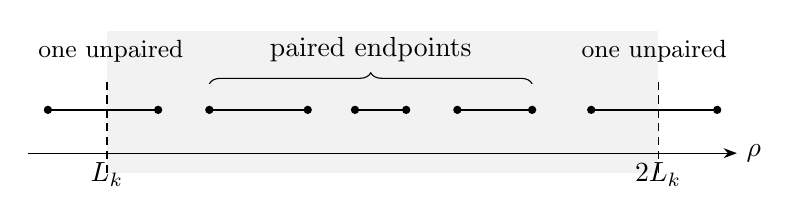
\begin{tikzpicture}[x=1cm,y=1cm,>=Stealth]
 \fill[gray!10] (1,-.25) rectangle (8,1.55);
 \draw[->] (0,0)--(9,0) node[right] {$\rho$};
 \draw[densely dashed] (1,-.25)--(1,.93);
 \draw[densely dashed] (8,-.25)--(8,.93);
 \node[below] at (1,0) {$L_k$};
 \node[below] at (8,0) {$2L_k$};
 \draw[thick] (.25,.55)--(1.65,.55);
 \draw[thick] (2.3,.55)--(3.55,.55);
 \draw[thick] (4.15,.55)--(4.8,.55);
 \draw[thick] (5.45,.55)--(6.4,.55);
 \draw[thick] (7.15,.55)--(8.75,.55);
 \foreach \x in {.25,1.65,2.3,3.55,4.15,4.8,5.45,6.4,7.15,8.75}
   \fill (\x,.55) circle (1.5pt);
 \draw[decorate,decoration={brace,amplitude=4pt}]
   (2.3,.88)--(6.4,.88);
 \node[above] at (4.35,1.04) {paired endpoints};
 \node[above,align=center,font=\small] at (1.05,1.03) {one unpaired};
 \node[above,align=center,font=\small] at (7.95,1.03) {one unpaired};
\end{tikzpicture}
\caption{Endpoint grouping inside one dyadic interval.  Intervals with
both endpoints in the group contribute differences; their total
length is at most $L_k$.  Only intervals reaching a boundary of the
dyadic interval can leave unpaired endpoints.  The picture is schematic.}
\label{fig:endpoint-pairing}
\end{figure}

For $|z|\le3$, first consider the smooth term
$s_\alpha(z)=P(|z|/\alpha)/z$ in \eqref{eq:dimensionless-endpoint}.
The function $P$ has a smooth even extension and vanishes quadratically
at zero.  Hence $s_\alpha$ extends smoothly across $z=0$, and
\[
 \sup_{\substack{|z|\le3\\1\le\alpha\le2}}
 \bigl(|\partial_\alpha s_\alpha(z)|
       +|\partial_z\partial_\alpha s_\alpha(z)|\bigr)<\infty.
\]
The fundamental theorem of calculus in $\alpha$, followed by
\eqref{eq:paired-length}, bounds the sum of the paired smooth terms
and their $z$-derivatives independently of their number.
For the hard terms, the paired difference is
\[
 -\frac{c_0}{z}
    \bigl(\mathbf1_{\{|z|>\alpha_j\}}
          -\mathbf1_{\{|z|>\gamma_j\}}\bigr).
\]
Away from endpoints, at most one such difference is nonzero at any
fixed $|z|$, because the intervals $(\alpha_j,\gamma_j)$ are disjoint.
On its support $|z|\ge1$, so its size and its classical derivative
are uniformly bounded.  The at most two unpaired terms have the
same bounds on this compact range.

For $|z|>3$, all indicators in \eqref{eq:dimensionless-endpoint}
equal one, and
\[
 P(|z|/\alpha)-c_0=-2g_3''(|z|/\alpha).
\]
Consequently $e_\alpha$, $\partial_z e_\alpha$,
$\partial_\alpha e_\alpha$, and
$\partial_z\partial_\alpha e_\alpha$ are bounded by
$Ce^{-cz^2}$, uniformly for $1\le\alpha\le2$.
The paired-length estimate and the two unpaired contributions prove
the same bound for their sum.  Combining the compact and tail
estimates proves \eqref{eq:paired-endpoint-bound}.

We finish by separating the groups according to their counts.
At each output point, \eqref{eq:endpoint-count} implies that there
are at most $2\sqrt n$ indices with $m_{a,b,k}>\sqrt n$.
The uniform Gaussian bound \eqref{eq:paired-endpoint-bound} and
Lemma~\ref{lem:gaussian-envelope} bound all these groups together,
after integration in $c$, by
$C\sqrt n\mathcal M_{F,G}(-a,-b)$.
Their trilinear contribution is at most
$C\sqrt n\prod_v\|G_v\|_3$.

Set the kernels and counts of those groups to zero.  The remaining
family satisfies \eqref{eq:rough-family-decay}, has odd kernels,
and has counts satisfying
$\sum_km_{a,b,k}\le2n$ and $m_{a,b,k}\le\sqrt n$.
Corollary~\ref{cor:odd-family} applies and proves
\eqref{eq:endpoint-error-bound}.  Every grouping and deletion is made
at the output point, so the proof imposes no common choice of
endpoints or dyadic groups at different output points.
\end{proof}

\section{From the count estimate to full variation}\label{sec:completion}

We now assemble the smooth estimate and the endpoint estimate, remove
the restrictions on choices and inputs, and sum the count bounds to
obtain the full variation. No selection of a common partition for
different output points is made in this argument.

\begin{proof}[Proof of Theorem~\ref{thm:count}]
First let $F,G\in C_c^\infty(\R^2)$, use the pair maps
\eqref{eq:pair-maps}, and take $G_0\in C_c^\infty(\R^2)$.
For step choices of disjoint annuli and coefficients, the identity
\eqref{eq:hard-smooth} writes the hard linearization, multiplied by
$c_0\ne0$, as its smooth linearization minus its endpoint errors.
Propositions~\ref{prop:smooth-switches} and~\ref{prop:endpoint-errors}
therefore give
\begin{equation}\label{eq:hard-linearized-bound}
 \left|\iiint G_0(a,b)G_1(b,c)G_2(c,a)
     \sum_j\frac{\beta_j\mathbf1_{\{\varepsilon_j<|a+b+c|<R_j\}}}
                       {a+b+c}\dd a\dd b\dd c\right|
 \le C\sqrt n\log(2+n)\prod_v\|G_v\|_3.
\end{equation}
The interval list and coefficients in the sum may vary with $(a,b)$.

Fix a finite menu of such choices. Its measurable choice sets can be
approximated in measure on a compact set by finite unions of rectangles.
To see this, approximate each of the finitely many sets using Lebesgue
regularity and then refine all rectangle boundaries to one coordinate
partition. Resolve overlaps by a fixed ordering of the menu; the total
mismeasured set remains bounded by the sum of the approximation errors.
Assign any menu item on the remaining cells. For the fixed menu, the
annuli are uniformly bounded away from zero, and the integrals against
the smooth inputs are bounded on the compact support needed for $G_0$.
Consequently the corresponding linearized integrals converge.
Thus \eqref{eq:hard-linearized-bound} holds for arbitrary measurable
choices from a fixed finite menu.

Now fix a finite collection of lists of disjoint rational annuli, each
of length at most $n$. The maximum of their sums of absolute increments
is measurable. Choose a maximizing list measurably by resolving ties in
a fixed order. For each of its increments choose a coefficient from
$\{1,-1,i,-i\}$ whose product with that increment has real part at least
half its modulus. These choices are again measurable and range over
a finite menu. Testing \eqref{eq:hard-linearized-bound} against
nonnegative smooth compactly supported $G_0$ shows, by $L^3$ duality,
that this finite maximum has $L^{3/2}$ norm at most
$C\sqrt n\log(2+n)\|F\|_3\|G\|_3$.
The reflection $(x,y)=(-a,-b)$ preserves that norm.
Exhausting the countable family of all rational lists and applying
monotone convergence proves the count bound for smooth inputs.

For general complex $F,G\in L^3$, choose smooth compactly supported
approximants $F_m,G_m$. For every fixed annulus, bilinearity and
\eqref{eq:finite-annulus-bound} give convergence of
$B_{\varepsilon,R}(F_m,G_m)$ in $L^{3/2}$.
For a fixed finite collection of lists, the difference of the two
finite maxima is bounded by a finite sum of such truncation differences.
It therefore converges in $L^{3/2}$. Pass the estimate to the limit
for this finite maximum, then exhaust the rational lists once more.
Lemma~\ref{lem:finite-truncations} supplies the common representatives
required in the definition of $\mathcal S_n$.
\end{proof}

\begin{proof}[Proof of Theorem~\ref{thm:variation}]
For any finite rational partition, arrange the absolute annular
increments in nonincreasing order, denoting them by
$d_1\ge d_2\ge\cdots\ge0$. Whenever the index $2^j$ exists,
the corresponding largest increments are a permissible list in
$\mathcal S_{2^j}$, so
\[
 d_{2^j}\le2^{-j}\mathcal S_{2^j}(F,G).
\]
The group of indices $2^j\le l<2^{j+1}$ has at most $2^j$ members.
Bounding the full $\ell^r$ norm by the sum of the group norms yields,
uniformly in the chosen partition,
\begin{equation}\label{eq:rank-variation}
 V_r(F,G)\le\sum_{j\ge0}2^{j/r-j}\mathcal S_{2^j}(F,G)
 \quad\text{almost everywhere}.
\end{equation}
Theorem~\ref{thm:count} and Minkowski's inequality now imply
\[
 \|V_r(F,G)\|_{3/2}
 \le C\|F\|_3\|G\|_3
       \sum_{j\ge0}(1+j)2^{j(1/r-1/2)}.
\]
The series converges for every $r>2$. In particular, neither a bound
on the number of increments nor a restriction to dyadic endpoints
survives in the conclusion.
\end{proof}

\section{Maximal estimates and principal values}\label{sec:consequences}

The counting estimate already contains the maximal estimate, by taking
a single annulus. We first record its continuity with respect to the
inputs, then use that continuity to transfer joint principal-value
convergence from smooth functions to all complex $L^3$ inputs.
Throughout this section, write $p=3/2$.

\begin{corollary}[The hard maximal operator]\label{cor:maximal}
For complex $F,G\in L^3(\R^2)$, define
\[
 B_*(F,G)(x,y)
 =\sup_{0<\varepsilon<R<\infty}|B_{\varepsilon,R}(F,G)(x,y)|
\]
on the common full-measure set of Lemma~\ref{lem:finite-truncations},
and set it to zero elsewhere. This function is measurable, and there is
an absolute constant $C_M$ such that
\begin{equation}\label{eq:hard-maximal-bound}
 \|B_*(F,G)\|_p\le C_M\|F\|_3\|G\|_3.
\end{equation}
The supremum includes both finite hard truncation endpoints. Moreover,
$B_*$ is a continuous map from $L^3(\R^2)\times L^3(\R^2)$ to
$L^p(\R^2)$ and is the unique continuous extension of its values on
compactly supported smooth pairs.
\end{corollary}

\begin{proof}
Endpoint continuity in Lemma~\ref{lem:finite-truncations} identifies the
supremum with its restriction to rational endpoint pairs. Consequently
it is measurable and equals $\mathcal S_1(F,G)$. Theorem~\ref{thm:count}
gives \eqref{eq:hard-maximal-bound}, with its absolute factor
$\log 3$ absorbed into $C_M$.

For two pairs of inputs, bilinearity of each finite truncation gives,
almost everywhere,
\begin{equation}\label{eq:maximal-continuity}
 |B_*(F,G)-B_*(f,g)|
 \le B_*(F-f,G)+B_*(f,G-g).
\end{equation}
Taking $L^p$ norms and using \eqref{eq:hard-maximal-bound} proves
continuity. Density of compactly supported smooth functions gives the
asserted uniqueness.
\end{proof}

\begin{corollary}[Joint bilinear principal values]\label{cor:bilinear-pv}
For every complex $F,G\in L^3(\R^2)$, the joint limit
\[
 B(F,G)=\lim_{\substack{\varepsilon\downarrow0\\R\uparrow\infty}}
 B_{\varepsilon,R}(F,G)
\]
exists almost everywhere and in $L^p(\R^2)$, and
\[
 \|B(F,G)\|_p\le C_M\|F\|_3\|G\|_3.
\]
More precisely, the entire tail converges in the maximal sense
\begin{equation}\label{eq:maximal-tail-convergence}
 \left\|\sup_{\substack{0<\varepsilon<1/n\\R>n}}
 |B_{\varepsilon,R}(F,G)-B(F,G)|\right\|_p
 \longrightarrow0.
\end{equation}
The operator $B$ is the unique bounded complex bilinear extension of
the principal-value operator on compactly supported smooth inputs.
\end{corollary}

\begin{proof}
For compactly supported smooth $f,g$ and fixed $(x,y)$, put
$h(t)=f(x+t,y)g(x,y+t)$. Then
\[
 B_{\varepsilon,R}(f,g)(x,y)
 =\int_\varepsilon^R\frac{h(t)-h(-t)}t\,\dd t.
\]
The numerator is $O(t)$ at zero and vanishes for large $t$, so the joint
limit exists at every point.

For general $F,G$, define the tail oscillation
\[
 \Omega_n(F,G)=
 \sup_{\substack{0<\varepsilon,\varepsilon'<1/n\\R,R'>n}}
 |B_{\varepsilon,R}(F,G)-B_{\varepsilon',R'}(F,G)|.
\]
These functions are measurable by endpoint continuity, decrease with
$n$, and satisfy $0\le\Omega_n(F,G)\le2B_*(F,G)$. Choose compactly
supported smooth $f_m\to F$ and $g_m\to G$ in $L^3$. Take a common
full-measure set for the pairs $(F,G)$, $(f_m,g_m)$, $(F-f_m,G)$,
and $(f_m,G-g_m)$, for all $m$. On this set, bilinearity gives
\[
 \Omega_n(F,G)\le\Omega_n(f_m,g_m)
       +2B_*(F-f_m,G)+2B_*(f_m,G-g_m).
\]
The smooth joint convergence implies $\Omega_n(f_m,g_m)\to0$ pointwise.
Thus, writing $\Omega_\infty=\lim_n\Omega_n(F,G)$, we obtain
\[
 \|\Omega_\infty\|_p
 \le2C_M\bigl(\|F-f_m\|_3\|G\|_3
             +\|f_m\|_3\|G-g_m\|_3\bigr).
\]
Letting $m\to\infty$ shows that $\Omega_\infty=0$ almost everywhere.
This is the joint Cauchy criterion for the two endpoints, and hence
defines $B(F,G)$ almost everywhere. Taking, for example, the cofinal
sequence $(\varepsilon,R)=(1/(2n),2n)$ shows that the limit is measurable;
its magnitude is at most $B_*(F,G)$. Define it to be zero on the
remaining null set.

Letting $(\varepsilon',R')$ tend jointly to $(0,\infty)$ in the
definition of $\Omega_n$ gives
\[
 \sup_{\substack{0<\varepsilon<1/n\\R>n}}
 |B_{\varepsilon,R}(F,G)-B(F,G)|\le\Omega_n(F,G).
\]
The supremum is measurable, again by endpoint continuity.
Dominated convergence applies because
$\Omega_n(F,G)\le2B_*(F,G)\in L^p$, proving
\eqref{eq:maximal-tail-convergence} and therefore joint norm convergence.
The norm bound follows from $|B(F,G)|\le B_*(F,G)$. Passing to the
$L^p$ limit in the bilinear identities for finite truncations proves
complex bilinearity. The bound and density then prove uniqueness.
\end{proof}

\subsection{Flat and simplex scalar forms}

For complex $F_0,F_1,F_2\in L^3(\R^2)$, let
\[
 \mathcal L_{\varepsilon,R}(F_0,F_1,F_2)
 =\iiint_{\varepsilon<|t|<R}
 F_0(x,y)F_1(x+t,y)F_2(x,y+t)
 \,\dd x\,\dd y\,\frac{\dd t}{t}.
\]
No input is conjugated in this scalar form.

\begin{corollary}[Flat scalar principal values]\label{cor:scalar-pv}
For every complex $L^3$ triple, each finite flat truncation is absolutely
integrable, and
\[
 \sup_{0<\varepsilon<R<\infty}
 |\mathcal L_{\varepsilon,R}(F_0,F_1,F_2)|
 \le C_M\prod_{v=0}^2\|F_v\|_3.
\]
Its joint scalar principal value exists and equals
$\int_{\R^2}F_0 B(F_1,F_2)$. This limiting form is the unique bounded
complex trilinear extension of its compactly supported smooth definition.
\end{corollary}

\begin{proof}
H\"older's inequality in $(x,y)$ bounds the integral of the absolute
value by $2\log(R/\varepsilon)\prod_v\|F_v\|_3$. Fubini's Theorem
therefore identifies the finite form with
$\int F_0 B_{\varepsilon,R}(F_1,F_2)$.
Corollary~\ref{cor:maximal} gives its uniform bound, and pairing the
joint $L^p$ limit in Corollary~\ref{cor:bilinear-pv} with $F_0$ gives
the scalar principal value. The limiting form is bounded and complex
trilinear; density proves uniqueness.
\end{proof}

In simplex coordinates the corresponding scalar form is
\[
 \Lambda_{\varepsilon,R}(G_0,G_1,G_2)
 =\iiint_{\varepsilon<|a+b+c|<R}
 G_0(a,b)G_1(b,c)G_2(c,a)
 \,\frac{\dd a\,\dd b\,\dd c}{a+b+c}.
\]
The equivalence of the flat and simplex formulations, including their
optimal constants, is described in
\cite[Appendix~B.1]{KovacThieleZorinKranich2015}. We record the
norm-preserving maps to track both hard endpoints and their joint limit.

\begin{proposition}[Scalar equivalence]\label{prop:flat-equivalence}
For every complex $G_0,G_1,G_2\in L^3(\R^2)$, each finite simplex
truncation is absolutely integrable, and
\[
 \sup_{0<\varepsilon<R<\infty}
 |\Lambda_{\varepsilon,R}(G_0,G_1,G_2)|
 \le C_M\prod_{v=0}^2\|G_v\|_3.
\]
Its joint scalar principal value exists and is the unique bounded
complex trilinear extension of its compactly supported smooth
definition. The optimal constants in the uniform finite flat and
simplex scalar estimates are equal.
\end{proposition}

\begin{proof}
Use the determinant-one change of variables
\[
 x=-a,\qquad y=-b,\qquad t=a+b+c,
 \qquad
 a=-x,\quad b=-y,\quad c=t+x+y.
\]
For flat inputs set
\[
 \begin{aligned}
 G_0(u,v)&=F_0(-u,-v),\\
 G_1(u,v)&=F_1(u+v,-u),\\
 G_2(u,v)&=F_2(-v,u+v).
 \end{aligned}
\]
Each pair map has determinant one. The inverse formulas are
\[
 \begin{aligned}
 F_0(r,s)&=G_0(-r,-s),\\
 F_1(r,s)&=G_1(-s,r+s),\\
 F_2(r,s)&=G_2(r+s,-r).
 \end{aligned}
\]
These maps preserve $L^3$ norms, compact smoothness, and the Schwartz
class. Direct substitution identifies both the integrands and the
finite truncation regions. Absolute integrability, the uniform bound,
and joint scalar convergence therefore follow from
Corollary~\ref{cor:scalar-pv}. The inverse maps realize every simplex
triple, so the optimal constants are equal. Density proves uniqueness
of the bounded trilinear extension.
\end{proof}

For completeness, let $C_S$ denote this common optimal scalar constant.
It is also the optimal constant for the uniform family of individual
bilinear bounds
\[
 \|B_{\varepsilon,R}(F,G)\|_p
 \le C_S\|F\|_3\|G\|_3.
\]
Indeed, H\"older's inequality gives one direction. For the other, if
$U\in L^p$ is nonzero, then
\[
 H=\frac{\overline U}{|U|}\,
       \frac{|U|^{1/2}}{\|U\|_p^{1/2}},
\]
defined to be zero where $U=0$, satisfies $\|H\|_3=1$ and
$\int HU=\|U\|_p$. Apply this duality formula to each finite bilinear
truncation. In particular, the optimal pointwise maximal constant is
at least $C_S$; equality of the scalar constants does not assert
equality with the maximal or variation constants.

\bibliographystyle{plain}
\bibliography{references}
\end{document}
